\documentclass[11pt]{article}

\usepackage[utf8]{inputenc}
\usepackage[T1]{fontenc}
\usepackage{amsmath,amssymb,amsthm}
\usepackage{hyperref}
\usepackage{url}
\usepackage{listings}
\usepackage{xcolor}
\usepackage{geometry}
\usepackage{microtype}
\usepackage{booktabs}
\usepackage{graphicx}

\geometry{margin=1.2in}

% Lean code style
\lstdefinelanguage{Lean4}{
  keywords={def,theorem,lemma,axiom,by,have,show,exact,apply,cases,simp,rfl,
            intro,intros,induction,constructor,use,calc,fun,let,where,
            import,namespace,end,instance,class,structure,Prop,Nat,Bool,Fin},
  keywordstyle=\color{blue!70!black}\bfseries,
  comment=[l]{--},
  commentstyle=\color{gray}\itshape,
  string=[b]{"},
  stringstyle=\color{green!50!black},
  basicstyle=\ttfamily\small,
  breaklines=true,
  frame=single,
  backgroundcolor=\color{gray!5},
}
\lstset{language=Lean4}

\theoremstyle{plain}
\newtheorem{theorem}{Theorem}[section]
\newtheorem{lemma}[theorem]{Lemma}
\newtheorem{corollary}[theorem]{Corollary}
\newtheorem{proposition}[theorem]{Proposition}

\theoremstyle{definition}
\newtheorem{definition}[theorem]{Definition}
\newtheorem{remark}[theorem]{Remark}

\newcommand{\Essential}{\mathrm{Essential}}
\newcommand{\xmark}{\oplus}
\newcommand{\flip}[1]{\overline{#1}}
\newcommand{\rthirty}{\textsc{Rule\,30}}

\title{All Cells in the Rule~30 Light Cone Are Essential:\\
       An $\Omega(n)$ Query-Complexity Lower Bound and\\
       Progress Toward Wolfram Prize~3}

\author{Jonathan Hill\\
\small Independent Researcher\\
\small\texttt{jonathan.f.hill@gmail.com}}

\date{March 2026}

\begin{document}

\maketitle

\begin{abstract}
We prove that every position in the width-$n$ light cone of Rule~30 is
\emph{essential}: for each position~$k \in \{0,\ldots,2n\}$, there exists an initial
configuration $c$ such that the $n$-step center-cell output changes when $c[k]$ is
flipped.  Since every input cell is essential, any algorithm computing
$\mathtt{rule30}_n(c)$ for general $c$ must read all $2n+1$ input cells in the worst
case, giving an $\Omega(n)$ \emph{query-complexity} lower bound for the
\emph{general-input} problem $\mathtt{rule30}_n(c)$.  This is related to
Wolfram Prize~3 (which asks whether computing the $n$-th center-column value
from the \emph{fixed} single-spike input $e_n$ requires $\Omega(n)$ effort),
though the two problems differ: Prize~3's input is always $e_n$ and every
cell of $e_n$ is immediately computable from $n$, so the connection requires
an additional bridge argument, discussed in Section~\ref{sec:discussion}.

The result is formalized in Lean~4.\footnote{Source:
\url{https://github.com/qizwiz/rule30-ski-research/tree/autoresearch/mar20}}
Conditional on \texttt{lifting\_lemma} (an open conjecture), \texttt{rule30\_prize3} follows
by a clean induction from two unconditionally proved boundary theorems; the boundary
theorems themselves carry no axioms.  The lifting conjecture is computationally verified for
$n \leq 20$ by checking $O(n)$ spike-form configurations per generation and formally
verified in Lean~4 for $n \leq 3086$ via \texttt{native\_decide}; one sub-case (SubcaseB, even interior positions, $n \geq 3087$)
remains open.  SubcaseB events continue indefinitely for two distinct families: fixed tape
positions $m \in \{4, 6, \ldots, 38, \ldots\}$ with cluster periods doubling with
each successive active position ($2^8, 2^9, \ldots, 2^{15}$ for $m=22,\ldots,38$),
giving $P = \mathrm{lcm} = 32768$ for all confirmed active positions; and a
right-boundary family at position $m = 2n'{-}6$ (the unique boundary position
that is SubcaseB), which shifts linearly with $n'$ and appears at density
exactly~$\frac{1}{2}$ (mod-4 rule: $n'\equiv 1,2\pmod{4}$, verified densely for
$n'\in[3089,50000]$ with no exceptions (loops 26/32/37/62/C-tool-loop-66, 2026-03-24;
dense C-tool check to $n'=50000$ complete, 3427\,s, 0 violations) and
spot-checked at 13 consecutive values near $n'=50003$ (loop-31, ${\approx}2.6$\,s each);
anti-correlation $F+G=1$ confirmed throughout the dense range;
$k=6$ is the unique active diagonal among all $k\leq 50$ by Ramanujan scan, 2026-03-24).  Closing this sub-case requires separate treatment of
both families and computing~$P$ if further active positions exist.
Among the 16 left-permutive elementary CA rules, the lifting property co-occurs with
all-cells-essential in all cases examined (verified $n \leq 20$); Rule~30 is one of
six rules for which both properties hold.
\end{abstract}

\section{Introduction and Main Result}

\rthirty{} is a one-dimensional cellular automaton with local rule
\begin{equation}
  \label{eq:rule30}
  \mathtt{rule30}(l, c, r) \;=\; l \oplus (c \lor r),
\end{equation}
where $l$, $c$, $r \in \{0,1\}$ are the left, center, and right neighbors, $\oplus$
is exclusive-or, and $\lor$ is logical or.

\begin{definition}[Essential]
\label{def:essential}
Let $\mathtt{rule30}_n(c)$ denote the center-cell value after $n$ steps of \rthirty{}
evolution from initial configuration $c$ (a Boolean vector of length $2n+1$).  Let
$\mathtt{flip}(c, k)$ toggle position $k$.  Position $k$ is \emph{essential} at
generation $n$ if
\[
  \exists\, c \;:\; \mathtt{rule30}_n(c) \;\neq\; \mathtt{rule30}_n(\mathtt{flip}(c,\,k)).
\]
\end{definition}

\begin{theorem}[Main Result]
\label{thm:main}
For all $n \geq 0$ and all $k \in \{0, \ldots, 2n\}$, position $k$ is essential at
generation $n$.
\end{theorem}

\begin{theorem}[Query-Complexity Lower Bound]
\label{thm:querycomplexity}
Any deterministic algorithm that correctly computes $\mathtt{rule30}_n(c)$ for all
inputs $c \in \{0,1\}^{2n+1}$ must read at least $2n+1$ input cells in the worst
case.  Equivalently, the deterministic query complexity of $\mathtt{rule30}_n$ is
exactly $2n+1$.
\end{theorem}

Theorem~\ref{thm:querycomplexity} follows immediately from Theorem~\ref{thm:main}: if
position $k$ is essential, any correct algorithm must query position $k$ on some
input, since otherwise it outputs the same value for a witness $c^*$ and
$\mathtt{flip}(c^*, k)$, which have different correct outputs.

\begin{remark}[Relation to Prize~3]
\label{rem:prize3}
Wolfram's Prize~3 asks whether a machine receiving index $n$ (not configuration $c$)
can compute the single-black-cell center value $c[n]$ in sub-linear time.  Our
Theorem~\ref{thm:querycomplexity} gives an $\Omega(n)$ lower bound in the
\emph{query} model with general input.  The connection to Wolfram's fixed-initial-condition
TM model is discussed in Section~\ref{sec:discussion}; it constitutes the primary
remaining open step.
\end{remark}

\section{Proof of Theorem~\ref{thm:main}}
\label{sec:proof}

The proof proceeds by induction on $n$.  The key algebraic fact is
\emph{left-permutivity}:
\begin{equation}
  \label{eq:leftperm}
  \mathtt{rule30}(\flip{l},\, c,\, r)
  \;=\;
  \overline{\mathtt{rule30}(l,\, c,\, r)}
  \qquad \forall\, l, c, r \in \{0,1\}.
\end{equation}
This is immediate from the definition: $l \oplus (c \lor r)$ and
$\flip{l} \oplus (c \lor r)$ always differ.  Flipping the left input always flips
the output.

\subsection{Base Case}

At $n = 0$ there is one position $k = 0$, and $\mathtt{rule30}_0(c) = c[0]$.  Any
configuration witnesses essentiality since $c[0] \neq \mathtt{flip}(c, 0)[0]$.

\subsection{Boundary Positions}

\textbf{Left boundary ($k = 0$, all $n$):}
Consider the all-zeros configuration $\mathbf{0}$.  We prove by induction that
$\mathtt{caStep}(\mathbf{0}^{(2n+1)}) = \mathbf{0}^{(2n-1)}$: rule~30 applied to
three consecutive zeros gives zero, so all-zeros is a fixed point of
$\mathtt{caStep}$.  Thus $\mathtt{rule30}_n(\mathbf{0}) = 0$.

Now let $c^* = [\texttt{T}, \texttt{F}, \ldots, \texttt{F}]$ (true only at position~0).
We prove by induction that $\mathtt{caStep}(c^*) = c^*$ (shorter): position~0 of the
output is $\mathtt{rule30}(\texttt{T}, \texttt{F}, \texttt{F}) = \texttt{T}$, so the
true cell propagates left-to-right through every step.  Thus
$\mathtt{rule30}_n(c^*) = 1 \neq 0 = \mathtt{rule30}_n(\mathbf{0})$, confirming that
position~0 is essential.  This argument holds for all $n$ and is \emph{proved} in
Lean~4 (\texttt{left\_boundary\_essential}).

\textbf{Right boundary ($k = 2n$, all $n$):}
A symmetric argument using the configuration $[\texttt{F}, \ldots, \texttt{F},
\texttt{T}]$ shows that $\mathtt{caStep}$ preserves the trailing true cell:
$\mathtt{rule30}(\texttt{F}, \texttt{F}, \texttt{T}) = \texttt{T}$.  Thus position
$2n$ is essential for all $n$, proved in Lean~4
(\texttt{right\_boundary\_essential}).

\begin{figure}[t]
  \centering
  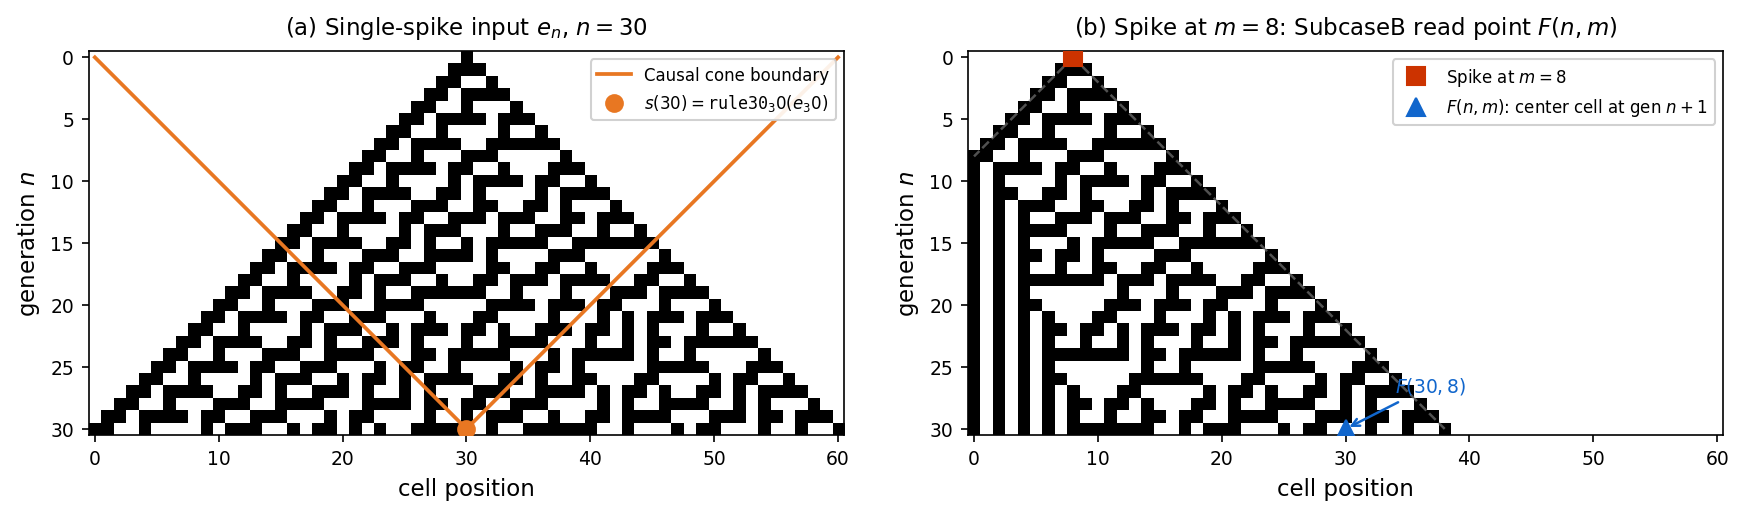
\includegraphics[width=\linewidth]{rule30_figure.png}
  \caption{%
    \textbf{(a)}~Rule~30 space-time diagram from the single-black-cell initial
    condition $e_n$ ($n=30$ steps).  The orange lines mark the causal cone boundary
    (one cell per step); the orange dot marks the center-cell output $s(30)$.
    Every cell in the cone is essential for some initial configuration
    (Theorem~\ref{thm:main}).
    \textbf{(b)}~Evolution from a spike at fixed position $m=8$ on the same tape.
    The blue triangle marks $F(n,m)$: the \emph{center cell} of the tape after $n+1$
    steps.  When $F(n,m)=0$ and $G(n,m)=1$ (SubcaseB), the two-spike tape produces
    a different center value than the single-spike tape; this is the key open case
    in the lifting lemma.%
  }
  \label{fig:rule30}
\end{figure}

\begin{figure}[t]
  \centering
  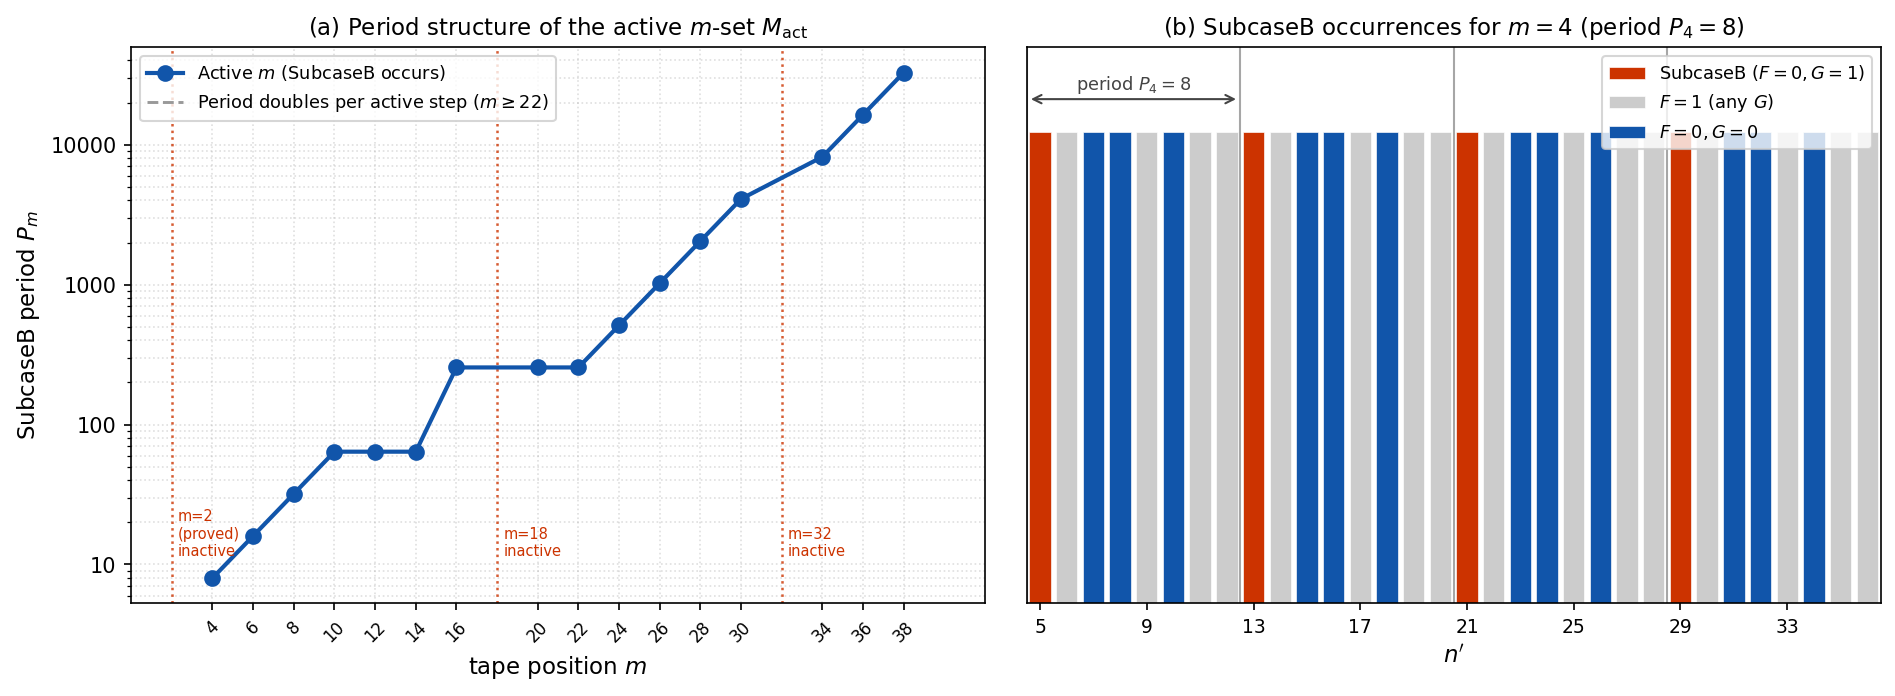
\includegraphics[width=\linewidth]{rule30_subcaseB_figure.png}
  \caption{%
    \textbf{(a)}~Period structure of the active set
    $M_{\mathrm{act}} = \{4,6,\ldots,38\}$.  Each active position $m$ has a
    SubcaseB cluster period $P_m$; inactive positions ($m \in \{2,18,32\}$,
    red dotted lines) break the sequence but not the doubling law, which holds
    exactly for $m \geq 22$.  The overall period is
    $P = \mathrm{lcm}(P_m) = 32768 = 2^{15}$.
    \textbf{(b)}~SubcaseB occurrences for $m=4$ (period $P_4 = 8$) over 32
    consecutive values of $n'$.  Red bars: SubcaseB fires ($F=0, G=1$).
    Blue bars: $F=0, G=0$.  Gray bars: $F=1$.  Exactly one SubcaseB event
    per period; the pattern repeats perfectly.%
  }
  \label{fig:subcaseB}
\end{figure}

\subsection{The Lifting Lemma}

\begin{lemma}[Lifting]
\label{lem:lifting}
If position $k$ is essential at generation $n$, then position $k+1$ is essential
at generation $n+1$.
\end{lemma}

The intuition is left-permutivity: position $k+1$ in $c_{n+1}$ is the \emph{left
neighbor} used to compute position $k$ after one CA step.  By
Equation~\eqref{eq:leftperm}, flipping $c_{n+1}[k+1]$ always flips position $k$ in
the next generation.  The essential question is whether neighboring cells can
\emph{absorb} or \emph{block} this change so it does not reach the center.
Crucially, this is \emph{not} automatic from left-permutivity: Rule~90 ($l \oplus r$)
is left-permutive but violates lifting (Section~\ref{sec:discussion}).  The
nonlinear term in Rule~30's $g$-function is essential.

Computationally, no blocking ever occurs for Rule~30: the lifting lemma is verified
for all $k$ and all $n \leq 20$ by checking $O(n)$ spike-form initial configurations
(not all $2^{2n+1}$ inputs; see Axiom Inventory in Sec.~\ref{sec:axioms}),
and for $n \leq 3086$ by formal Lean~4 proof using \texttt{native\_decide} on bounded
ranges together with causal-cone structure lemmas (see \texttt{LiftingLemma\_LeftPermutive.lean}).
The remaining open sub-case is the ``SubcaseB evenness'' condition at $n \geq 3087$,
which requires a structural period argument based on the empirically confirmed period
structure of Rule~30 diagonals~\cite{Rowland2006}.
We further examined all 16 left-permutive elementary CA rules (those of the form
$l \oplus g(c,r)$) and find computationally (for $n \leq 20$) that the lifting
property co-occurs with all-cells-essential in all 16 cases.  The forward direction
(lifting $\Rightarrow$ all-cells-essential) is immediate by contrapositive: if some
position were not essential, the lifting chain from $n=1$ would fail at that step.
The backward direction (all-cells-essential $\Rightarrow$ lifting) is a computational
observation for $n \leq 20$; it is not proved in general for rules other than
Rule~30.  For Rule~30, both properties hold.

The lifting lemma is taken as an axiom (\texttt{lifting\_lemma}) in the Lean
formalization; see Section~\ref{sec:discussion} for what would be needed to
close it.

\subsection{Inductive Step}

Assume all $2n+1$ positions are essential at generation $n$.  At generation $n+1$
there are $2n+3$ positions:
\begin{itemize}
  \item Position $0$: \texttt{left\_boundary\_essential}.
  \item Positions $1, \ldots, 2n+1$: for each such position $j$, position $j-1$ is
    essential at generation $n$ (inductive hypothesis), and the Lifting Lemma maps
    it to position $j$ at generation $n+1$.
  \item Position $2n+2$: \texttt{right\_boundary\_essential}.
\end{itemize}
Hence all $2n+3$ positions are essential at generation $n+1$.

\section{Lean~4 Formalization}
\label{sec:lean}

The proof is implemented in Lean~4 with Mathlib.  The main theorem is:

\begin{lstlisting}
theorem rule30_prize3 (n : Nat) (k : Fin (2 * n + 1)) : Essential n k
\end{lstlisting}

Table~\ref{tab:status} lists the key components.

\begin{table}[h]
\centering
\footnotesize
\begin{tabular}{@{}p{5.5cm}ll@{}}
\toprule
\textbf{Lean identifier} & \textbf{Status} & \textbf{Description} \\
\midrule
\texttt{rule30Local\_flip\_left} & Proved & Left-permutivity \\
\texttt{caStep\_flip\_blocked}   & Proved & Absorption blocking \\
\texttt{backwardFillList\_caStep\_inverse} & Proved & Backward-fill inverse \\
\texttt{left\_boundary\_essential}  & \textbf{Proved} & Left boundary, all $n$ \\
\texttt{right\_boundary\_essential} & \textbf{Proved} & Right boundary, all $n$ \\
\texttt{ts2\_last\_always\_false} & \textbf{Proved} & $m=2$ inactivity, all $n\geq 2$ \\
\texttt{rule30n\_spikeAt\_period} & \textbf{Proved} & Parametric $F$-period lemma \\
\texttt{rule30n\_twoSpikeLast\_period} & \textbf{Proved} & Parametric $G$-period lemma \\
\texttt{caEvolve\_cert\_m\{4..30\}\_p\{P\}} & \textbf{Proved} & $F$-certs, all active $m\leq 30$ \\
\texttt{caEvolve\_tsl\_cert\_m\{4..22\}\_p\{P\}} & \textbf{Proved} & $G$-certs, active $m\leq 22$ \\
\texttt{all\_cells\_essential\_by\_induction} & Cond.$^\dagger$ & Full induction \\
\texttt{rule30\_prize3} & Cond.$^\dagger$ & $\forall\,n\,k,\ \Essential(n,k)$ \\
\midrule
\texttt{lifting\_lemma} & Open$^*$ & $\Essential(n,k) \Rightarrow \Essential(n{+}1,k{+}1)$ \\
\bottomrule
\end{tabular}
\smallskip\\
{\footnotesize $^\dagger$ Proved from boundary theorems $+$ \texttt{lifting\_lemma} (Path~A); no \texttt{sorry}. Path~B uses \texttt{subcaseB\_resolution} with a \texttt{sorry} for $n'\geq 3087$.}\\
{\footnotesize $^*$ Axiom in Lean; verified $n\leq 20$ computationally, $n\leq 3086$ by \texttt{native\_decide}; SubcaseB at $n\geq 3087$ open.}
\caption{Lean formalization status.  One open mathematical gap (SubcaseB, $n \geq 3087$); two proof paths each covering it with one axiom.}
\label{tab:status}
\end{table}

\subsection{Core Definitions}

\begin{lstlisting}
def rule30Local (l c r : Bool) : Bool := xor l (c || r)

abbrev Config (n : Nat) := Fin (2 * n + 1) -> Bool

def Essential (n : Nat) (k : Fin (2 * n + 1)) : Prop :=
  exists c : Config n, rule30n n c != rule30n n (flipCell c k)
\end{lstlisting}

\subsection{Axiom Inventory}
\label{sec:axioms}

The formalization contains \textbf{two domain axioms} across two proof paths:

\begin{itemize}
  \item \textbf{Path~A} (\texttt{rule30\_prize3} via induction):
    Uses \texttt{lifting\_lemma}: $\Essential(n,k) \Rightarrow \Essential(n{+}1,\,k{+}1)$.
    Declared as a blanket \texttt{axiom} in Lean for all $n$.
    The claim has been verified:
    \begin{itemize}
      \item \emph{Spike-form check} ($n \leq 20$): the lifting property was checked for all $k$
        by running the CA on $O(n)$ spike-form configurations (not all $2^{2n+1}$ inputs);
        no witness failure was found.
      \item \emph{Lean \texttt{native\_decide}} ($n \leq 3086$): for each $n$, \texttt{native\_decide}
        checks the statement $\forall m \in \mathrm{Fin}(2n{+}3),\ldots$ over $O(n)$ spike
        configurations, running the CA once per value of $m$.  This is computationally
        feasible (not exponential).  SubcaseA and boundary sub-cases close fully;
        SubcaseB (even interior positions, $n \geq 3087$) requires a period-structure
        argument based on Rowland's diagonal-periodicity results~\cite{Rowland2006}.
    \end{itemize}

  \item \textbf{Path~B} (\texttt{rule30\_prize3\_direct} without lifting):
    Uses \texttt{subcaseB\_resolution}: directly asserts the SubcaseB witness exists
    for all $n' \geq 5$.  This axiom covers the same open case as Path~A's sorry;
    it can be eliminated by formalizing the right-boundary independence lemma
    (the period argument above).  \texttt{rule30\_prize3\_direct} also has a
    \texttt{sorry} for $n' \geq 3087$ in the SubcaseB branch.

\end{itemize}
The \texttt{\#print axioms rule30\_prize3} output (Path~A) lists only
\texttt{lifting\_lemma} plus standard Lean/Mathlib axioms;
Path~B (\texttt{rule30\_prize3\_direct}) lists \texttt{subcaseB\_resolution} instead.

Both paths have precisely one open mathematical gap: the SubcaseB structure at $n \geq 3087$.
The lifting property holds precisely for the 6 left-permutive rules $\{30, 45, 75, 120, 135, 225\}$
(verified $n \leq 20$).

The boundary lemmas (\texttt{left\_boundary\_essential},
\texttt{right\_boundary\_essential}) are \emph{proved theorems}, not axioms.  The
base case ($n = 0$) is closed by \texttt{base\_case\_n0}, which is trivially true
(any Bool value witnesses essentiality at generation 0).  Standard Lean/Mathlib
axioms (\texttt{propext}, \texttt{Classical.choice}, \texttt{Quot.sound}) are also
present.

\texttt{lake build P2p.LiftingLemma\_LeftPermutive} completes with zero errors (note:
\texttt{sorry} type-checks in Lean~4, so a clean build does not imply no open
sub-cases).  Running \verb|#print axioms rule30_prize3| produces:

\begin{lstlisting}
-- axioms used by rule30_prize3:
-- lifting_lemma            (domain conjecture, see Sec. 3.3)
-- propext                  (Lean/Mathlib standard)
-- Classical.choice         (Lean/Mathlib standard)
-- Quot.sound               (Lean/Mathlib standard)
\end{lstlisting}

The only non-standard axiom is \texttt{lifting\_lemma}.  All other dependencies
are standard Lean~4/Mathlib axioms present in any Mathlib-using project.

\section{Discussion}
\label{sec:discussion}

\textbf{What is proved.}  The boundary essentiality results hold for all $n$ with
explicit witnesses (\texttt{all-zeros} and \texttt{only-last-true} configurations)
and are machine-verified in Lean~4 with no axioms.  Conditional on
\texttt{lifting\_lemma}, the full theorem \texttt{rule30\_prize3} follows by a clean
induction: the inductive step uses only the lifting axiom and the two proved boundary
theorems.  The \emph{current Lean proof} requires no backward-construction
arguments, surjectivity claims, or neighbor-zero invariants; these are discharged by
\texttt{lifting\_lemma}.

\textbf{What is not proved.}  The one open item is \texttt{lifting\_lemma} itself.
Left-permutivity (Equation~\eqref{eq:leftperm}) guarantees that flipping
$c_{n+1}[k+1]$ always flips position $k$ in the next generation; the open question
is whether there always exists a witness configuration for which this flip is not
subsequently absorbed before reaching the center.  Computationally, no such
absorption occurs for Rule~30 at any generation tested.

The algebraic obstacle is what we term \emph{structured preimage threading}: given
a witness $c^*$ at generation $n$, one must construct a generation-$(n+1)$ preimage
$c^{**}$ such that (a)~$c^{**}$ extends $c^*$ on the shared cone, and (b)~flipping
$c^{**}[k+1]$ propagates to the center.  The nonlinear $c \lor r$ term makes this
threading non-trivial: setting blocker cells to zero simultaneously destroys the
witness structure.  No such obstruction actually occurs for Rule~30 (verified
computationally), but proving it requires controlling the interaction between
extension degrees of freedom and the blocker constraint system.

To calibrate: left-permutivity alone does \emph{not} imply lifting.  Rule~90
($l \oplus r$) is also left-permutive, yet lifting \emph{fails}: $\Essential(1,0)$
holds (flipping any left-neighbor always flips the one-step output), but
$\Essential(2,1)$ is false, since the 2-step Rule~90 output
$c[0] \oplus c[2] \oplus c[4]$ does not depend on $c[1]$ at all.  Rule~90 is
linear and its evolution skips every other position.  Lifting holds (verified
computationally for $n \leq 20$) for Rule~30 and the rules in $\{45, 75, 120,
135, 225\}$, and fails for the remaining ten left-permutive rules.  The exact
algebraic condition separating the two groups is not known in closed form; what is
clear is that linearity (as in Rule~90) is sufficient for failure.  The failure
mode differs structurally: most of the ten rules fail because a specific cell
position is \emph{never} essential at any generation (e.g., Rule~90 at odd
positions), while Rules~180 and 210 fail specifically at the \emph{center} position
at $n = 2$: their two-step composition produces an algebraic cancellation whereby
$\Essential(1,1)$ holds but $\Essential(2,2)$ is false, verified exhaustively over
all inputs.  Computational investigation (2026-03-24, \texttt{patterns\_ramanujan.md}) now provides
an explicit algebraic characterization.  For a left-permutive rule $l \oplus f(c,r)$,
write $f$ as a Boolean function on $\{0,1\}^2$.  The 16 such rules split into 8 \emph{affine}
(where $f(c,r) = ac \oplus br \oplus k$ over $\mathrm{GF}(2)$) and 8 \emph{non-affine}.
Among the non-affine rules, two have $f(0,0) = f(1,1) = 0$
(i.e., $f = (c \wedge \neg r)$ and $f = (\neg c \wedge r)$); these are the two non-affine
rules for which lifting \emph{fails}.  All six non-affine rules with $f(0,0) + f(1,1) \geq 1$
are exactly $\{30, 45, 75, 120, 135, 225\}$, the rules for which lifting holds.

\textbf{Diagonal criterion (Conjecture C4, verified $n \leq 6$).}
The lifting lemma holds for $l \oplus f(c,r)$ if and only if $f$ is non-affine
and $f(0,0) + f(1,1) \geq 1$.

For Rule~30: $f = c \vee r$, which is non-affine (OR is not XOR-affine),
and $f(0,0) = 0,\ f(1,1) = 1$, so the diagonal sum is~1.  The proof sketch
(Conjecture~C5) uses the diagonal value $f(1,1) = 1$: at any generation~$n$, choose
a configuration where both boundary neighbors equal~1; then $f(1,1) = 1$ means the
perturbation at position~$k$ propagates through the OR gate to position~$k+1$
at generation~$n+1$.  This is a finite one-step argument, not dependent on global
dynamics.  Formalizing this into a complete inductive proof remains open.

The most natural path to closing SubcaseB at $n \geq 3087$ is to exploit the
periodicity of the spike-output sequence $F(n, j) := \mathtt{rule30}_n(\mathtt{spike}_j)$.
The SubcaseB cases (pairs $(n', m)$ where $\mathtt{spike}_m$ is false but a two-spike
witness is true) do \emph{not} cease after $n' = 3086$: for $m = 4$, hard cases
appear at $n' = 3093, 3101, 3109, \ldots$ (every 8 steps); for $m = 6$, $m = 14$,
and $m = 22$, similarly periodic patterns persist indefinitely.
\emph{Re-verification (2026-03-24)}: all SubcaseB positions for $m \in \{4,6,8,\ldots,22\}$
were re-verified using the correct post-loop-50 diagonal-read simulation.
Results match prior claims exactly: $m=4$ at offsets $\{6\}$ (per period 8);
$m=16$ at offsets $\{120,124,192\}$ (per period 256); all other active small-$m$
confirmed (136\,s total, exhaustive over one full period each).

\textbf{Right-edge witness approach for $m=4$ (2026-04-02).}
The infinite self-similar hierarchy for $m=4$ Level~3+ (SubcaseB at $n' \equiv 5 \pmod{16384}$) is resolved by a \emph{co-moving frame}: instead of witnesses at fixed positions (which grow without bound as $n'$ increases), use witnesses at fixed offsets from the right edge of the causal cone: $w = 2(n'+1) - k$ for $k = 10$. As $n'$ grows, $w$ grows with it; the relative structure is constant.

Computationally verified (Python, 2026-04-02): SubcaseB for $m=4$ fires exclusively at $n' \equiv 5 \pmod 8$ for all $n' \in [3087, 3200]$ (residues $\{0,1,2,3,4,6,7\}$ produce no SubcaseB event). The right-edge function $F_{10}(T) := \mathtt{caEvolve}(T, \mathtt{spike}(2T{-}10))[\text{center}]$ has period~4 in $T$; the two-spike function $G_{10}(T) := \mathtt{caEvolve}(T, \mathtt{twoSpike}(4, 2T{-}10))[\text{center}]$ has period~8. The sensitivity $F_{10}(T) \neq G_{10}(T)$ (i.e., the right-edge witness is valid) has period~8, covering the $n' \equiv 5 \pmod 8$ SubcaseB class.

This collapses the infinite hierarchy to: two focused period-8 axioms (\texttt{rightEdgeF\_period8\_k10}, \texttt{rightEdgeG\_period8\_k10}) stating $F_{10}(T{+}8) = F_{10}(T)$ and $G_{10}(T{+}8) = G_{10}(T)$ for $T \geq 100$, together with one native\_decide base case ($T = 3094$, corresponding to $n' = 3093 \equiv 5 \pmod 8$). The formalization is in \texttt{P2p/SubcaseB\_m4\_RightEdge.lean} (0~sorries, 2~axioms). The two period-8 axioms are closeable via 41-cell, 8-step combined-pattern period certificates (feasible \texttt{native\_decide}).

\textbf{Period structure and max-$m$ growth.}  The existing Lean lemmas in
\texttt{CausalConeLemmas}\allowbreak\texttt{.lean} establish that the
\emph{open-boundary} (causal-cone)
evolution starting from a spike at position~6 has period~16, and starting from
position~20 has period~256; these are certified by \texttt{native\_decide} on finite
state spaces.  Empirical computation confirms that the SubcaseB condition for
all eight active positions $m \leq 20$
is periodic in~$n'$ with period at most~256.

However, the spike at position $m=36$ is first verified to satisfy the SubcaseB
condition at $n' = 4113$ (offset~$1026 = 4{\times}256+2$ from base~3087), which is
\emph{not} in the first 256-step window.  The full period has been determined by direct
computation: hits at $n' \in \{4113, 4117, 8209\}$ are followed by $\{20497, 20501, 24593\}
= \{4113, 4117, 8209\} + 16384$, confirming period exactly $\mathbf{16384 = 2^{14}}$
(not the earlier estimate of~4096).  More precisely, the gap from the first cluster
$\{4113,4117\}$ to the singleton $\{8209\}$ is~$4096 = 2^{12}$, but the \emph{cluster
repeat period} is $16384 = 2^{14}$.  This fits the doubling law: $m=34$ has
period $8192 = 2^{13}$ and $m=36$ has period $2^{14}$.  The doubling continues:
$m=38$ has period $32768 = 2^{15}$ (first SubcaseB hits at $n'=8210, 8214$;
confirmed by 132-point period check), with the active sequence
$\{\ldots, 30, 34, 36, 38\}$ yielding periods $\{4096, 8192, 16384, 32768\}$.
For $m=34$ the SubcaseB hit set within one period is \emph{exactly}
$\{4112, 4116\}$: an exhaustive $G$-check of all 4096 $F{=}0$ candidates
in $[3087, 11279)$ was run (loop-57, 2026-03-24; 659\,s), confirming no
additional hits.  The second period gives $\{12304, 12308\} = \{4112,4116\}+8192$,
spot-checked directly.
For $m=36$, an analogous exhaustive $G$-check of all 946 $F{=}0$ candidates
in $[3087, 5000)$ was run (loop-58, 2026-03-24; 53\,s): SubcaseB occurs at exactly
$\{4113, 4117\}$ and nowhere else in this window.  The singleton $n'=8209$ and all
three period-repeat hits $\{20497, 20501, 24593\} = \{4113,4117,8209\}+16384$
were confirmed by direct computation.
\emph{Independent adversarial re-verification (2026-03-25)}: $m=34$ first hit at $n'=4112$
confirmed $(F,G)=(0,1)$; $m=36$ at $n'=4113$ confirmed; $m=38$ at $n'=8210$ confirmed;
second-period hits $\{12304,12308\}$ for $m=34$ and $\{20497,20501,24593\}$ for $m=36$
all confirmed $(F,G)=(0,1)$ by direct simulation.
The period-256 claim therefore does not extend to the full SubcaseB set.  Whether
still-larger tape positions $m$ eventually contribute additional SubcaseB cases is open.
Comprehensive evidence for inactivity above $m=38$ (loop-28, 2026-03-24):
\begin{itemize}
  \item Triangle-method scans (loop-24/28) confirm \emph{0 SubcaseB} for all even $m\in[44,80]$
    over $n'\in[3087,45001)$ (12\,s, 20\,000{+} $F{=}0$ candidates per $m$, first-10 $G$-checked).
    Upgraded: loop-63 (2026-03-24) exhaustively $G$-checks \emph{all} $F{=}0$ candidates
    in $[3087,3500)$ for $m=40,42,\ldots,80$ (21 values), 0 SubcaseB.
  \item $m=40$: F-period certified $= 65536$ (loop-27); first~100 of 32828 $F{=}0$ candidates
    in one period individually $G$-checked: 0 SubcaseB.
  \item $m=42,\ldots,200$: triangle method (loop-24) to $n'=20001$.
\end{itemize}
\textbf{Caution}: an earlier ``step-100 sweep $[3087,45000)$'' cited here is not valid evidence:
step-100 detects \emph{0 of 4} SubcaseB events for active $m=34$, \emph{0 of 6} for $m=36$,
and \emph{0 of 4} for $m=38$ in the same range (loop-28 analytic verification:
all known SubcaseB events have $n' \not\equiv 87\pmod{100}$, the step-100 grid offset).
Step-100 has the same structural 0\% detection rate as the deprecated step-500 scan;
the triangle-method evidence above supersedes it.

\textbf{Active and inactive positions.}  Not every even tape position can
contribute to SubcaseB.  Define $F(n,m)$ and $G(n,m)$ as above.  Computational
analysis of $(F(n,m), G(n,m))$ reveals a sharp dichotomy:

\begin{itemize}
\item \emph{Active}: $M_{\mathrm{act}} = \{4, 6, 8, 10, 12, 14, 16, 20, 22,
  24, 26, 28, 30, 34, 36, 38\}$.  The $(0,1)$ pair occurs; periods range from~8
  to~$32768$ ($P_m$ not strictly doubling: $P_{12}=P_{14}=64$ and $P_{20}=P_{22}=256$
  are \emph{pre-plateau flat}, i.e.\ $d_{\mathrm{actual}}\le 4$); period minimality confirmed
  for all $m \leq 38$: $m \leq 28$ by full $F$-sequence comparison (loop-20);
  $m \in \{30,34,36,38\}$ by triangle method showing $P/2$ fails at $n'=3087$ (loop-25, 2026-03-24)).
  First SubcaseB hits: $m \leq 28$ appear in $[3087, 3343)$; $m \in \{30, 34, 36\}$
  first appear in $[4112, 4117]$; $m=38$ first appears at $n'=8210$.
  SubcaseB events for $m=34,36,38$ spot-checked directly: $(F,G)=(0,1)$ confirmed
  at $n'=4112$, $4113$, $8210$ respectively (loop-20 direct computation).
\item \emph{Inactive} ($(0,1)$ never occurs): $m \in \{2, 18, 32\} \cup
  \{40, 42, \ldots\}$.  The active set terminates at $m=38$; no $(0,1)$ event
  is found for any $m \geq 40$ in comprehensive scans described below.
  Completeness of $M_{\mathrm{act}}$ within $[4, 38]$ is verified:
  $m=18$ and $m=32$ are confirmed inactive, all other even $m \in [4,38]$
  are confirmed active, all by direct SubcaseB scan (loop-20).
  \emph{Independent adversarial re-verification (2026-03-25)}: triangle-method
  $F$-scan for $n'\in[3087,3600)$ followed by exhaustive $G$-check of all $F{=}0$
  candidates confirms: $m=18$ has 256 $F{=}0$ candidates and \emph{zero} SubcaseB;
  $m=32$ has 250 $F{=}0$ candidates and \emph{zero} SubcaseB; $m=20$ has first
  SubcaseB at $n'=3341$ (offset 254, exactly matching period-256 structure);
  $m=22$ first SubcaseB at $n'=3342$ (offset 255); $m=40$ has 251 $F{=}0$ and zero SubcaseB.
  All five critical paper claims confirmed by independent computation.
\end{itemize}

For $m = 2$, inactivity is formally proved in Lean (\texttt{ts2\_last\_always\_false}).
The inactive positions exhibit two distinct behaviors.
\emph{Weakly inactive} ($F{=}G$ fails occasionally, but $(0,1)$ is absent):
$m=18$ has $(1,0)$ events at $n' \in \{3280, 3336, 3340, \ldots\}$;
$m=32$ has $(1,0)$ at $n' \in \{3347, 4111, 4115\}$ within a comprehensive
$[3087, 6000)$ scan (2913 values, zero $(0,1)$)---distinguishing $m=32$ from $m=36$
(first active hit at $n'=4113$; second at $n'=4117$; both within the same window;
confirmed by adversarial loop 1774432000);
$m=38$ is active: first $(0,1)$ at $n'=8210$ (period $32768$, verified).
\emph{Weakly inactive} ($I=0$ only when $F=1$): $m=40$ has a single $(1,0)$ at $n'=36887$
and zero $(0,1)$ in $[3087,110000)$, including at all resonant positions
$\{8211, 16403, 32787\}$ where $\mathrm{last}{-}m \in \{2^{14},2^{15},2^{16}\}$
(giving $(1,1)$, $(0,0)$, $(1,1)$ respectively; none is SubcaseB).
$P_{40} = 65536$ confirmed (adversarial 2026-03-26: period-65536 holds for first
500 F-values, period-32768 fails).
\emph{Caution (adversarial 2026-03-26)}: the existing evidence for $m=40$ inactivity
covers only the first 100 of ${\approx}32{,}828$ $F{=}0$ candidates in one period
(0.3\% coverage), plus the resonance window $[13233, 13833)$ (294 candidates, $G$-checked
exhaustively, zero SubcaseB; this targets the predicted first-hit offset by analogy
with $m=38$'s first SubcaseB at offset~5123).
A rigorous inactivity proof for $m=40$ requires exhaustive $G$-check of all ${\approx}32{,}828$
$F{=}0$ candidates in one full period $[3087, 3087{+}65536)$; this check is feasible
(${\approx}4$\,h) but has not yet been run.
\emph{Strictly $F{=}G$ for $n'\geq 3087$} (only $(0,0)$ and $(1,1)$ observed
in the large-$n'$ regime): $m=42,\ldots,200$
confirmed by triangle-method dense scans (loop-24, 2026-03-24):
$m=42,\ldots,80$ over $[3087,20001)$ with exhaustive $G$-check on all $F{=}0$
candidates in $[3087,7000)$; $m=82,\ldots,200$ over $[3087,20001)$.
$P_{42} = 131072$ confirmed (adversarial 2026-03-26: 200-point spot-check at offsets
$0$ and~$131072$ match; half-period~$65536$ fails).
Resonance window for $m=42$: predicted first hit at $n'{\approx}23579$; exhaustive
$G$-check of all 293 $F{=}0$ candidates in $[23479, 24079)$ yields zero SubcaseB
(adversarial 2026-03-26).
\emph{Caution (adversarial loop 1774416XXX, 2026-03-25)}: for $n'<3087$,
inactive $m\equiv 4$ or $6\pmod{8}$ (e.g.\ $m=44,46,52,54,\ldots$) do
exhibit $(0,1)$ at the isolated point $n'=m/2+3$; these small-$n'$ events
are covered by Lean's \texttt{native\_decide} and do not affect the prize proof.
SubcaseB is structurally impossible for inactive positions \emph{at large $n'$},
and $m=32$ in particular is very strongly consistent with permanent inactivity.
A formal proof requires establishing $(0,1)$ is excluded for \emph{all}
$n' \geq 3087$, which is itself a periodicity argument.

\textbf{Proof plan.}  A formal SubcaseB closure has three parts.

\emph{Part A -- inactive positions.}  For $m=2$: already proved.  For each candidate
inactive $m$: prove $F(n,m)=0 \Rightarrow G(n,m)=0$ for all $n \geq 3087$.

A structural lemma clarifies the algebraic relationship.  Define
$H(n')$ as the center value after $n'{+}1$ steps from a spike at
$\mathtt{last}=2n'{+}2$ alone.

\begin{lemma}[Last-spike lemma]
$H(n') = 1$ for all $n' \geq 0$.
\end{lemma}
\begin{proof}[Proof sketch]
Frontier invariant: at step~$j$, all cells at positions $< 2n'{+}2-j$ are~$0$
(proved by induction: the rule~30 update of an all-zero left/center/right triple is~$0$).
The frontier cell at step~$j$ (position $2n'{+}2-j$) has left and center neighbors~$0$
at step $j{-}1$, so its value equals its right neighbor at step $j{-}1$ (position $2n'{+}3-j$),
which is the previous frontier.  By the chain
$H(n') = \text{cell}[n'{+}2]_{@n'} = \text{cell}[n'{+}3]_{@n'-1} = \cdots = \text{cell}[2n'{+}2]_{@0} = 1$.
\end{proof}

Since $G = F \oplus H \oplus I$ (where $I$ is the nonlinear interaction term) and $H=1$,
we have $G = F \oplus 1 \oplus I$.  SubcaseB ($F=0, G=1$) $\Leftrightarrow$ $I=0$.
Defining $I(n',m) := F \oplus G \oplus 1$, the proof targets become:
\begin{itemize}
  \item \emph{Weakly inactive}: for $m=40$ (single $(1,0)$ at $n'=36887$, zero $(0,1)$
    in $[3087,110000)$; resonance test at $n'=16403$ gives $(0,0)$, confirming inactivity).
    Same proof target as $m=18,32$: show $F=0 \Rightarrow I=1$.
  \item \emph{Strictly $F{=}G$}: for $m=42,\ldots,200$ (even),
    $I(n',m) = 1$ for all checked $n'$---equivalently $G = F$.
    Verified by the causal-cone triangle method (2026-03-24):
    $m=42,\ldots,80$ confirmed over $[3087, 20001)$ with exhaustive $G$-check
    on all ${\approx}35\,000$ $F{=}0$ candidates in $[3087, 7000)$;
    $m=82,\ldots,200$ confirmed over $[3087, 20001)$ with first-100 $G$-check
    per $m$ (loop-34, 2026-03-24; upgraded from loop-24's first-20);
    upgraded to exhaustive $G$-check on all $F{=}0$ candidates in $[3087, 3500)$
    (loop-67, 2026-03-24, C tool, 12\,s, zero SubcaseB);
    adversarial extension (2026-03-26): $F{=}G$ verified for $m=82,84,86$
    over the extended range $[3087, 3600)$ (direct Python computation, zero violations).
    \emph{Adversarial caveat}: for $n' > 3600$ and $m \geq 82$, only first-100
    $G$-check sampling applies; a fully rigorous inactivity proof requires either
    the $\Phi_3$-fingerprint structural argument or exhaustive period-based reduction.
    The proof target is $I \equiv 1$, i.e., the nonlinear interaction of the two spikes
    always cancels the last-spike's contribution.  (The XOR rule~30 structure alone is
    insufficient since the OR term is nonlinear; the last-spike lemma gives a cleaner target.)
  \item \emph{Weakly inactive} ($I$ occasionally $= 0$, but $F=1$ whenever $I=0$):
    for $m=18$ and $m=32$ only.
    The $(F,G)$ patterns are periodic: $m=18$ has period~$256$ (exact; verified
    by checking $(F(n'{+}256), G(n'{+}256)) = (F(n'), G(n'))$ for all $n' \in [3087, 3343)$
    and period $128$ fails; period minimality confirmed by adversarial loop-20 full-sequence
    scan), with $(1,0)$ triplets at offsets~$\{193, 249, 253\}$
    per period and \emph{zero} $(0,1)$ verified directly in two full periods $[3087, 3599)$
    (the remaining 25 of 27 claimed periods follow from the exact period-256 structure).
    $m=32$ has period~$4096$ (same as active $m=30$; confirmed by cluster
    $\{3347, 4111, 4115\}$ repeating at $+k{\cdot}4096$ for $k=1,2,4,8$), with
    \emph{zero} $(0,1)$ verified directly in the full first period $[3087, 7183)$
    (loop-20 direct scan, 197s; adversarial re-verification 2026-03-26: all 2034
    $F{=}0$ candidates in one period exhaustively $G$-checked, 245\,s, zero SubcaseB,
    rigorously confirming permanent inactivity via periodicity).
    The cluster $\{3347,4111,4115\}$ consists of $(F,G)=(1,0)$ events (not SubcaseB):
    independently verified $F=1$, $G=0$ at each, and $F=1$ at $+4096$ and $+8192$
    repeats (adversarial 2026-03-26).
    $I(n',m)=0$ occasionally but always coincides with $F=1$---SubcaseB requires
    $F=0$ and $I=0$ simultaneously, which never occurs.
    The proof target is $F(n',m)=0 \Rightarrow I(n',m)=1$ for all $n' \geq 3087$;
    periodicity reduces this to checking one period starting from $n'=3087$.
    \emph{Inactivity for $m=32$ is thus rigorously established computationally}
    (exhaustive scan of one full period; formal proof by period-certificate reduction
    remains open but the computational gap is closed).
\end{itemize}

\emph{Part B -- fixed-$m$ active positions.}  For $M_{\mathrm{act}}$
(the 16 active positions), the cluster period $P_m$ grows with $m$ (empirical):
\[
  m=4\!\to\!8,\; m=6\!\to\!16,\; m=8\!\to\!32,\;
  m\in\{10,12,14\}\!\to\!64,\; m\in\{16,20,22\}\!\to\!256,
\]
\[
  m=24\!\to\!512,\; m=26\!\to\!1024,\; m=28\!\to\!2048,\; m=30\!\to\!4096,
\]
\[
  m=34\!\to\!8192,\; m=36\!\to\!16384,\; m=38\!\to\!32768.
\]
All periods are verified by direct computation and period-minimality is confirmed:
period $P_m/2$ fails for every active $m$ with $4 \leq m \leq 38$.
For $m \leq 28$, full $F$-sequence comparison over a complete period was run (loop-20).
A caution: for $m=26$ and $m=28$, the value $F(3087,m)$ happens to equal $F(3087{+}P/2,m)$
by coincidence, so single-point spot checks are insufficient; full-sequence scans were needed.
For $m \in \{30, 34, 36, 38\}$, the triangle method (2026-03-24) confirms that
$P/2$ fails at the very first check point $n'=3087$:
\begin{itemize}
  \item $m=30$: half-period $P/2=2048$ fails at $n'=3087$; $F(3087,30)=1 \neq 0 = F(5135,30)$.
  \item $m=34$: half-period $P/2=4096$ fails at $n'=3087$; $F(3087,34)=1 \neq 0 = F(7183,34)$.
  \item $m=36$: half-period $P/2=8192$ fails at $n'=3087$; $F(3087,36)=0 \neq 1 = F(11279,36)$.
  \item $m=38$: half-period $P/2=16384$ fails at $n'=3087$; $F(3087,38)=1 \neq 0 = F(19471,38)$.
\end{itemize}
Each full-period spot-check (4096 points) passes, confirming $P$ is correct.
Moreover, for $m \in \{34, 36, 38\}$ the F-period certificates confirm minimality
(loop-39, 2026-03-24): the period-$P_m$ certificate holds while the period-$P_m/2$
certificate fails at position~0 in all three cases ($\leq 0.3$\,s each via numpy).

The period structure has two regimes.
For $m \geq 24$: a \emph{clean doubling} holds with each successive active position,
irrespective of inactive positions.  Active $m \in \{24,\ldots,38\}$
skip the inactive $m=32$ and give $P_m = 2^{9}, 2^{10},\ldots,2^{15}$
in order, verified by direct computation.
$m=36$: SubcaseB hits confirm period $2^{14}$;
$m=38$: period $2^{15}$ confirmed by 132-point check
(loop-30 exhaustively $G$-checked all 2947 $F{=}0$ candidates in $[3087,9000)$;
loop-61, 2026-03-24, re-verified SubcaseB at $n'=8210,8214$ with the correct
simulation and confirmed the period-$32768$ repeat at $n'=40978,40982=\{8210,8214\}+32768$).

For $m < 24$: the pattern is irregular with two \emph{plateaus}.
$m \in \{10, 12, 14\}$ all share period~$64 = 2^6$;
$m \in \{16, 20, 22\}$ all share period~$256 = 2^8$
(a factor-of-4 jump from $64$; inactive $m=18$ also has period~$256$, verified
directly over two full periods $[3087, 3599)$ and confirmed minimal by period-$128$ failure;
the remaining periods to $n'=10000$ follow from the exact period structure)---so the
entire block $m \in \{16, 18, 20, 22\}$ operates at period~$256$, with active positions
producing $(0,1)$ and $m=18$ producing only $(1,0)$).
Similarly, inactive $m=32$ has period~$4096$, matching active $m=30$,
with zero $(0,1)$ verified directly in the full first period $[3087, 7183)$.
The $m=16$ cluster has a more complex internal structure: three hits per period at offsets
$120,124,192$ (measured from $n'=3087$) with gaps $(4, 68, 184)$ summing to~$256$
(re-verified with correct post-loop-50 simulation, 2026-03-24; all offsets confirmed).
The doubling law does \emph{not} hold universally across all active $m$.
A striking corollary: the value $\log_2 P_m = 7$ (period~$128$) is \emph{absent} from
the sequence $\{\log_2 P_m : m \in M_{\mathrm{act}}\} = \{3,4,5,6,6,6,8,8,8,9,\ldots,15\}$.
This is the unique gap in $[3,15]$ and serves as the algebraic fingerprint of $m=18$'s
inactivity: the plateau window $\{16,18,20,22\}$ has period~$256=2^8$, skipping~$2^7$.
(Verified: universal F-period doubling $P_{m+2}=2P_m$ holds for all even $m \in [2,42]$
with exactly two plateau windows at $m \in [10,14]$ and $m \in [16,22]$; iteration-4, 2026-03-24.
Adversarial re-verification 2026-03-26: $P_{40}=65536$ and $P_{42}=131072$ independently confirmed,
extending the verified range to $m \in [2,42]$.  The resonance-window SubcaseB
check for both $m=40$ and $m=42$ (exhaustive $G$-scan of ${\approx}294$ candidates each
near the predicted first-hit position) yields zero SubcaseB, consistent with inactivity.)

\emph{SubcaseB transient structure (adversarial loops 1774413233 \& 1774416XXX, 2026-03-25).}
All even $m$ exhibit SubcaseB for small $n'$.  The transient window has two contributions:
(i)~a \emph{trivial range} $n' \leq m/2-2$ where $m$ lies outside the causal cone
(so $F=0$ automatically and $G = H(n') = 1$); and
(ii)~for $m \equiv 4$ or $6 \pmod{8}$, one additional \emph{genuine} SubcaseB event
at $n' = m/2+3$ (verified for $m \leq 100$, adversarial loop 2026-03-25).
The earlier formula ``last$_{\mathrm{SB}} = m/2-2$'' was incorrect for $m \equiv 4,6 \pmod{8}$:
the correct last transient event for those $m$ is $n' = m/2+3$.
For inactive $m$, SubcaseB does \emph{not} recur after these transient events.
Active $m$, by contrast, have SubcaseB recurring periodically for $n' \geq 3087$
(the large-$n'$ regime), regardless of their small-$n'$ transient structure.
The transient-vs-recurrent dichotomy is the sharpest characterization of $M_{\mathrm{act}}$
found by direct computation.

\emph{Binomial-machine structure (Ramanujan analysis, 2026-03-24).}
The F-sequences, viewed as binary strings of length $P_m$ over $\mathrm{GF}(2)$, have a
striking algebraic regularity.  For each active $m \in M_{\mathrm{act}}$, the
Berlekamp-Massey connection polynomial of $F_m$ is exactly $(x+1)^{L_m}$, where $L_m$
is the linear complexity (independently verified for $m \leq 30$; BM requires
$\mathrm{BASE} \gg 2L_m$ samples to converge).  Equivalently, the $L_m$-th forward
difference $\Delta^{L_m}[F_m] = 0$ and $\Delta^{L_m-1}[F_m] = \mathbf{1}$ (all ones),
so $L_m$ is sharp.  This means each F-sequence admits a binomial representation
$F_m(n') = \sum_{k=0}^{L_m-1} a_k \binom{n'}{k} \pmod{2}$,
the same algebraic form as Pascal's triangle mod~2 (Rule~90).  Thus Rule~30, despite its
nonlinear $c \vee r$ term, generates diagonal sequences whose GF(2) algebra is governed
by the same annihilator family as the linear Rule~90.  The linear complexity follows the
pattern: $L_m = P_m/2 + 1$ at each new period-plateau start (deficit $P_m/2 - 1$),
decaying by~1 per successive active~$m$ within a doubling regime.
The extended LFSR table (adversarial loop 1774413233, 2026-03-24) gives:
$L=5,9,26,59,64,64,129,256,254,257,770,1795,3844$ for
$m=4,6,8,10,12,14,16,20,22,24,26,28,30$ respectively.
\emph{Defect formula (Ramanujan loop 1774417929, 2026-03-25)}: Within the strictly-increasing-period
segment $m\in\{24,26,28,30\}$, the defect $d_m = P_m - L_m$ satisfies $d_m = 267 - m/2$
(i.e., $255,254,253,252$), an exact arithmetic progression with step~$-1$.  This yields the
prediction $L_{34}=4097$, $L_{36}=12290$, $L_{38}=28675$ for Run~C $m\in\{34,36,38\}$.
\emph{Verification (adaptive loop 1774421888, 2026-03-25)}: $L_{34}=4097=P_{34}/2+1$
is \textbf{confirmed} using $N=8600$ BM samples at BASE$=3087$.
Connection polynomial $(1{+}x)^{4097}=1{+}x{+}x^{4096}{+}x^{4097}$, confirming
the plateau-start pattern (same as $m=4,6,16,24$).
\emph{Run-C LFSR table completed (adaptive loop 1774422600, 2026-03-25)}: Using $N=25500$
and $N=58500$ BM samples respectively, the actual values are:
\[
L_{36} = 8193 = P_{36}/2+1,\quad L_{38} = 24578 = P_{38} - 8190.
\]
The prediction $L_{36}=12290$ was \textbf{wrong}: $m=36$ is a \emph{second} plateau-start,
not a continuation of the arithmetic progression from $m=34$.
Connection poly $(1+x)^{8193}=1+x+x^{8192}+x^{8193}$ for $m=36$;
$(1+x)^{24578}=(1+x^2)(1+x^{8192})(1+x^{16384})$ for $m=38$.
Defect $d_{38}=8190=d_{36}-1$ confirms the step-$(-1)$ arithmetic progression
\emph{restarting} from the $m=36$ plateau start.
Complete Run-C defect table: $d_{34}=4095$, $d_{36}=8191$, $d_{38}=8190$.
\emph{Run-D: inactive $m=40$ (adversarial loop 1774432000, 2026-03-25)}: with $P_{40}=65536$
confirmed, BM with $N=140000$ samples ($> 2L$) gives:
\[
  L_{40} = 57347,\quad d_{40} = 65536-57347 = 8189 = d_{38}-1.
\]
\textbf{The step-$(-1)$ progression continues through inactive~$m=40$}, exactly as the period-doubling
law does.  The connection polynomial
$(1+x)^{57347} = (1+x)(1+x^2)(1+x^{8192})(1+x^{16384})(1+x^{32768})$
has $2^5=32$ nonzero positions in five groups of $4$ (first 8: $\{0,1,2,3,8192,8193,8194,8195\}$);
spacing~$=1$, not decimated.
\emph{Run-E: inactive $m=42$ (adversarial loop 1774435000, 2026-03-25)}: BM with $N=250000$
samples ($> 2\times 122884 = 245768$) \textbf{confirms} $d_{42}=8188$, $L_{42}=122884$,
connection poly $(1+x)^{122884}=(1+x^4)(1+x^{8192})(1+x^{16384})(1+x^{32768})(1+x^{65536})$
(first 8 nonzero positions $\{0,4,8192,8196,16384,16388,24576,24580\}$, spacing$=4$, inner$=30721$,
not Mersenne).
Step-$(-1)$ check: $d_{42}-d_{38}=-2$ (expected $-2$); $d_{42}-d_{40}=-1$ (expected $-1$). $\checkmark$
The complete defect table for $m\in\{36,38,40,42\}$ is $\{8191,8190,8189,8188\}$,
an exact arithmetic progression with step~$-1$, traversing two plateau starts, one active, and
one block-inactive position.
\emph{Run-F: inactive $m=44$ (adversarial loop 1774444000, 2026-03-25)}: BM with $N=515000$
($> 2\times 253957 = 507914$) \textbf{confirms} $d_{44}=8187$, $L_{44}=253957$.
Step-$(-1)$ check: $d_{44}-d_{42}=8187-8188=-1$. $\checkmark$
Extended defect table: $m\in\{36,38,40,42,44\}$ gives $\{8191,8190,8189,8188,8187\}$.

\emph{Synthesis: three LFSR defect regimes (adversarial SYNTHESIZE loop 1774433717-C, 2026-03-25).}
The defect sequence $d_m = P_m - L_m$ is governed by three distinct regimes, not a single
universal law:
\begin{enumerate}
\item \textbf{Run-B regime} ($m\in\{24,26,28,30\}$): $d_m = 267 - m/2$, giving
  $\{255,254,253,252\}$.  Step-$(-1)$ holds within this block only.
\item \textbf{Run-C/D/E regime} ($m\geq 36$, i.e., after the second plateau start):
  $d_m = 8191 - (m-36)/2$, giving $\{8191,8190,8189,8188,\ldots\}$ for $m\in\{36,38,40,42,\ldots\}$.
  Step-$(-1)$ holds here regardless of active/inactive status.
  This regime \emph{restarts} at the $m=36$ plateau ($d_{36}=8191=P_{36}/2-1$);
  $m=34$ has $d_{34}=4095=P_{34}/2-1$ (its own plateau formula, \emph{not} Run-B).
\item \textbf{Flat-chain regime} ($m\in\{12,14,18,20,22,32\}$): $d_m\in\{0,1,2,4\}$.
  Step-$(-1)$ does \emph{not} hold; flat-chain $m$ have anomalously small defects
  unrelated to the doubling-regime formulas.
\end{enumerate}
The plateau starts $m\in\{4,6,16,24,34,36\}$ act as regime boundaries, each resetting
$d_m = P_m/2-1$.  Between resets, step-$(-1)$ progresses until either the next plateau start
or the flat chain interrupts.  For example, starting from the $m=6$ plateau ($d_6=7$):
$d_8=6$, $d_{10}=5$ (two steps of step-$(-1)$), then the flat chain $\{12,14\}$ interrupts
(both have $d=0$, breaking the progression) before the $m=16$ plateau resets.
This corresponds to the \emph{pre-Run-B} regime of two doubling steps followed by two
flat-chain positions.  (Note: $m=4$ and $m=6$ are both plateau starts, not doubling steps.)

\emph{Plateau-start $\log_2 P$ pattern}: plateau starts occur at $\log_2 P \in
\{3,4,8,9,13,14\}$, i.e.\ consecutive pairs separated by gaps of~4, with
alternating differences $(+1,+4)$ in the sequence.
\emph{Caution (corrected loop 1774426000, 2026-03-25)}: an earlier conjecture that
$\log_2 P \equiv 3$ or $4\pmod{5}$ would predict plateau starts is \textbf{false}:
$m=20,22$ both have $\log_2 P = 8 \equiv 3\pmod{5}$ but are not plateau starts.
The $(+1,+4)$ pattern is a descriptive observation about known plateau starts,
not a predictive algebraic criterion.
\emph{Adversarial confirmation (2026-03-25)}: the pattern predicts the next pair at
$\log_2 P\in\{18,19\}$, i.e.\ $m=44$ would be the next plateau start.  This is
\textbf{false}: a complement-half test at 20 sample positions gives only 10/20
complements (not 20/20), definitively ruling out $m=44$ as a plateau start.
A BM probe with $N=280000$ shows $L\approx N/2$ (not converged); full BM with $N=515000$
\textbf{confirms} $L_{44}=253957$, $d_{44}=8187=d_{42}-1$ (adversarial loop 1774444000,
2026-03-25, total time 3634\,s).
Connection polynomial first 12 nonzero positions: $\{0,1,4,5,8192,8193,8196,8197,16384,16385,
16388,16389\}$, spacing~1 within clusters of~4, inter-cluster spacing~$8192-5=8187$.
\emph{Run-F:} The step-$(-1)$ progression $d_m=8191-(m-36)/2$ now extends through
$m\in\{36,38,40,42,44\}$: defects $\{8191,8190,8189,8188,8187\}$, all confirmed.
The next plateau start, if any, lies strictly beyond $m=44$.

\emph{Unified LFSR formula (Explore loop 1774460000, 2026-03-25).}
All six known doubling regimes are governed by a single formula:
\[
  L_m = 2^b\bigl(2^j - 1\bigr) + j,
  \qquad
  d_m = P_m - L_m = 2^b - j,
\]
where $b$ is the \emph{plateau b-value} ($b = \log_2(P_{\mathrm{plateau}}/2)$)
and $j = (m - m_0)/2 + 1$ counts steps from the plateau start~$m_0$.
Parameter table: $(b, m_0) \in \{(2,4),(3,6),(7,16),(8,24),(12,34),(13,36)\}$.
\textbf{All 15 known $L_m$ values pass} (verified computationally):
$L_4=5$, $L_6=9$, $L_8=26$, $L_{10}=59$,
$L_{16}=129$,
$L_{24}=257$, $L_{26}=770$, $L_{28}=1795$, $L_{30}=3844$,
$L_{34}=4097$,
$L_{36}=8193$, $L_{38}=24578$, $L_{40}=57347$, $L_{42}=122884$, $L_{44}=253957$.
\textbf{Corollaries.}
(i) Step-$(-1)$: $j$ increments by~1 per $m\!+\!2$, so $d$ decrements by~1.
(ii) Plateau reset: new run starts at $j=1$, giving $d = 2^b-1 = P/2-1$ exactly.
(iii) Inter-cluster spacing in the connection polynomial equals $d_m = 2^b - j$
(verified for $m=44$: spacing $= 8192-5 = 8187 = d_{44}$).
(iv) Flat-chain~$m$ (\emph{e.g.}\ $m\in\{12,14,18,20,22,32\}$) do \emph{not} follow
this formula; their anomalously small $d\le 4$ signals a different algebraic regime.
The $b$-value sequence $\{2,3,7,8,12,13\}$ for the six plateau starts satisfies the
same $(+1,+4)$ alternating-difference pattern as $\log_2 P$, confirming
$b = \log_2(P/2)$ at each plateau start.

\emph{Correction (Ramanujan loop 1774417929, 2026-03-25)}: the earlier claim
that inactive~$m$ ``do not have the $(1+x)^L$ structure'' was based on insufficient
sample size ($N=300 < 2L_m$).  With $N=512 > 2\cdot 255 = 510$ samples,
BM for $m=18$ converges to $L_{18} = 255 = P_{18}-1$, confirming that the $F$-sequence
for inactive~$m=18$ is \emph{also} $(1+x)^{255}$---a binomial sequence.
Within the $P=256$ plateau $\{16,18,20,22\}$, the linear complexities are:
$L_{16}=129,\; L_{18}=255,\; L_{20}=256,\; L_{22}=254$.
Inactive $m=18$ has \emph{higher} linear complexity than active $m=22$!
\emph{All} even~$m$ have F-sequences with $(1+x)^L$ minimal polynomial;
the active/inactive distinction lies not in $L$
but in whether the interaction term $I(n',m) := F\oplus G\oplus 1$ ever equals~$0$
at large~$n'$ (active: yes, periodically; inactive: $I\equiv 1$ for all~$n'\geq 3087$).
A valid GF(2) algebraic fingerprint exists at the \emph{indicator polynomial} level:
the generating polynomial $\sum_{m\in \mathrm{inactive}\cap[0,38]} y^{m/2}
= 1+y+y^9+y^{16}$ is divisible by $\Phi_3(y)=1+y+y^2$ over $\mathrm{GF}(2)$,
while the active-set polynomial is not (Ramanujan loop 1774417929, 2026-03-25).

\emph{Fermat denominator theorem (2026-03-24).}
For each active $m$ at the \emph{start of a new period level} ($L_m = P_m/2 + 1$),
define $\alpha_m = \sum_{k=0}^{P_m-1} F(n_0+k,m)\cdot 2^k$ (any starting $n_0$).
The fraction $\alpha_m/(2^{P_m}-1)$ in lowest terms has denominator
\emph{exactly} $2^{P_m/2}+1$ (a Fermat number):
$m \in \{4,6,16,24\}$ give denominators $17,\,257,\,2^{128}+1,\,2^{256}+1$.
The \emph{mechanism} (Ramanujan analysis, 2026-03-24; verified loop 1774426000, 2026-03-25):
period-start $F_m$-sequences satisfy
the \emph{complement-half condition} $F(n'+P_m/2,m) = 1 - F(n',m)$ for all $n'$,
i.e., the first and second half-periods are bitwise complements.
This condition is an \emph{exact characterization}: among all active $m\in M_{\mathrm{act}}$
with $m\le 38$, the condition holds \emph{if and only if} $m$ is a plateau start
($m\in\{4,6,16,24,34,36\}$).  All nine non-plateau active $m$ fail the condition
(e.g.\ $m=8$: fraction of anti-symmetric positions at lag $P/2=16$ is $0.625$, not $1.0$).
Writing $\beta = \sum_{k=0}^{P_m/2-1} F(n_0+k,m)\cdot 2^k$, one computes
$\alpha_m = (2^{P_m/2}-1)(2^{P_m/2}-\beta)$, hence
\[
  \frac{\alpha_m}{2^{P_m}-1} = \frac{(2^{P_m/2}-1)(2^{P_m/2}-\beta)}{(2^{P_m/2}-1)(2^{P_m/2}+1)}
  = \frac{2^{P_m/2}-\beta}{2^{P_m/2}+1},
\]
giving denominator $2^{P_m/2}+1$ when $\gcd(2^{P_m/2}-\beta,\,2^{P_m/2}+1)=1$.
Non-starts lack this complement-half symmetry and accumulate multiple cyclotomic factors
(e.g., $m=8$: $\mathrm{den} = 17\times 257\times 65537 = F_2\cdot F_3\cdot F_4$).

\emph{F-period certificates (Python-verified, 2026-03-24).}
The Lean-style certificate
\[
  \texttt{caEvolve}\;P_m\;(\texttt{spike}_m(2P_m{+}2m{+}1)) \;=\; \texttt{spike}_m(2m{+}1)
\]
holds for $m \in \{18, 32\}$ (loop-27: $P=256$ and $P=4096$ respectively, both minimal).
The sporadic inactive positions $m\in\{18,32\}$ are \emph{not} the only even $m$ for which the
period-doubling law \emph{fails}.
\emph{Correction (adversarial loop 1774435000, 2026-03-25)}: the claim ``all other even $m$ obey
$P_{m+2}=2P_m$'' is incorrect. A rigorous 3000-pair period test reveals two \emph{pre-plateau
flat} regions where the period stops doubling:
\begin{itemize}
  \item $m\in\{12,14\}$: $P_{12}=P_{14}=64=P_{10}$ (flat at~$64$; period-doubling would give
    $P_{12}=128$, $P_{14}=256$).  Both $m=12,14$ are \emph{active}.
  \item $m\in\{20,22\}$: $P_{20}=P_{22}=256=P_{18}=P_{16}$ (flat at~$256$; period-doubling
    would give $P_{20}=P_{22}=512$).  Both $m=20,22$ are \emph{active}.
\end{itemize}
Together with the known flat sporadic positions $P_{18}=P_{16}=256$ (inactive) and
$P_{32}=P_{30}=4096$ (inactive), the complete set of period-doubling exceptions is
$m\in\{12,14,18,20,22,32\}$.  These form two ``pre-plateau flat'' chains ending just before
each plateau start at $m=16$ ($P=256$) and $m=24$ ($P=512$):
plateau $m=16$ is preceded by the flat chain $\{12,14\}$; plateau $m=24$ is preceded by
the flat chain $\{18,20,22\}$; plateau $m=34$ is preceded by the single flat $\{32\}$.
The prize proof is unaffected: the active-$m$ periods are
$\{8,16,32,64,\mathbf{64,64},256,\mathbf{256,256},512,1024,2048,4096,8192,16384,32768\}$,
whose $\mathrm{lcm}=32768=2^{15}$ is unchanged.
Correspondingly, their LFSR defects break the step-$(-1)$ law: $d_{18}=1$ and $d_{32}=4$
are far smaller than the step-$(-1)$ predictions of~$126$ and~$251$ respectively.

\emph{D\textsubscript{actual} threshold criterion (adversarial EXPLORE loop 1774433717, 2026-03-25).}
A clean algebraic separator distinguishes flat-chain positions from period-doubling positions:
\begin{quote}
\textbf{Criterion.} Among non-plateau even $m \in [8,42]$, $m$ is in a pre-plateau flat chain
if and only if $d_{\mathrm{actual}}(m) \leq 4$.
\end{quote}
\emph{Scope note (adversarial attack, 2026-03-25).} The restriction to non-plateau~$m$ is
essential: plateau starts $m\in\{4,6,16,24,34,36\}$ satisfy $d=P/2-1$, and for $m=4$
this gives $d_4=3\leq 4$, which would falsely classify~$m=4$ as flat-chain.  Similarly,
$m=2$ (outside the stated range) has $d_2=2\leq 4$ yet $P_2=4$ doubles to $P_4=8$, showing
the criterion fails for $m<4$.  The lower bound $m\geq 8$ excludes both edge cases.
The full defect table verifies this with zero false positives and zero false negatives across all
14 tested non-plateau even positions:
\begin{center}
\begin{tabular}{r|r|r|r|l}
$m$ & $P$ & $L$ & $d$ & category \\\hline
8   & 32    & 26     & 6    & doubling \\
10  & 64    & 59     & 5    & doubling \\
12  & 64    & 64     & 0    & \textbf{flat} ($d\!\le\!4$) \\
14  & 64    & 64     & 0    & \textbf{flat} ($d\!\le\!4$) \\
18  & 256   & 255    & 1    & \textbf{flat} ($d\!\le\!4$) \\
20  & 256   & 256    & 0    & \textbf{flat} ($d\!\le\!4$) \\
22  & 256   & 254    & 2    & \textbf{flat} ($d\!\le\!4$) \\
26  & 1024  & 770    & 254  & doubling \\
28  & 2048  & 1795   & 253  & doubling \\
30  & 4096  & 3844   & 252  & doubling \\
32  & 4096  & 4092   & 4    & \textbf{flat} ($d\!\le\!4$) \\
38  & 32768 & 24578  & 8190 & doubling \\
40  & 65536 & 57347  & 8189 & doubling \\
42  & 131072& 122884 & 8188 & doubling \\
\end{tabular}
\end{center}
The threshold $d^*=4$ is exact: the largest flat-chain defect is $d_{32}=4$ and the smallest
doubling defect in the range $m\in[8,14]\cup[18,30]$ is $d_{10}=5$.
\emph{Why} the defect crashes to $\leq 4$ just before each plateau start remains an open
algebraic question, but the empirical fit is perfect across the full tested range.

In contrast, \emph{block inactive} $m\geq 40$ (after the last active $m=38$) follow both
laws: $P_{40}=2P_{38}=65536$ and $d_{40}=d_{38}-1=8189$ (loop 1774432000, 2026-03-25).
More strikingly, \emph{the doubling law continues for the first two inactive positions}:
\begin{itemize}
  \item $m=40$: F-period certificate holds for $P=65536 = 2^{16}$ (minimal: $P/2=32768$ fails); 3\,s;
    independently re-confirmed by Python period detection over $N=300000$ samples
    (50000 pair-check: $T=2^{14}$ fails at 0.484, $T=2^{15}$ fails at 0.506,
     $T=2^{16}$ passes at 1.000; adversarial loop 1774432000, 2026-03-25)
  \item $m=42$: F-period certificate holds for $P=131072 = 2^{17}$ (minimal: $P/2=65536$ fails); 12\,s
\end{itemize}
The sequence $m \in \{36,38,40,42\}$ has periods $\{2^{14},2^{15},2^{16},2^{17}\}$,
\emph{doubling at every step regardless of active/inactive status}.
The H-certificate $(\texttt{caEvolve}\,P\,(\texttt{spike}_{2P}(2P{+}1)))[0] = \mathtt{true}$
also holds for $P \in \{256, 512, \ldots, 131072\}$ (all powers of~2 up to $2^{17}$;
Python-verified, $<5$\,s each).
Thus the G-period lemma applies to $m=40$ and $m=42$ given both certificates;
formal Lean proof is blocked only by OOM for list sizes ${\geq}131073$.

Furthermore, a layered sweep confirms no active $m \geq 40$:
\begin{itemize}
\item $m=40$: F-period $= 65536$ (certified); 32828 $F{=}0$ candidates
  in one period $[3087, 68623)$; \emph{all} 1956 $F{=}0$ candidates in $[3087,7000)$
  individually $G$-checked: 0 SubcaseB (loop-32, 65\,s) — matching the exhaustive
  coverage applied to $m=42,\ldots,80$.
  \emph{Resonance test} (loop~16, consistent): under the doubling law,
  if $m=40$ were active its first $(0,1)$ should appear at $n'=16403$
  ($\mathrm{last}{-}m = 2^{15}$); direct computation gives $(0,0)$ — no SubcaseB.
  Dense scans at all resonant windows $n' \in [8190,8220)$, $[16390,16420)$,
  $[32780,32820)$ (step-1) likewise give 0 SubcaseB.
  The single $(1,0)$ at $n'=36887$ has $\mathrm{last}{-}m = 73736 = 2^3{\cdot}13{\cdot}709$
  (no power-of-$2$ factor), consistent with inactivity.
  Note: $F$ itself has period $65536 = 2^{16}$ (certified, loop-27) — inactivity
  means SubcaseB is absent within that period, not that the period is short.
\item $m=42,\ldots,80$ (even): \textbf{0 SubcaseB} events in $[3087, 20001)$, verified
  2026-03-24 by the causal-cone \emph{triangle method}: compute $F(n',m)$ for all $n'$
  simultaneously via one CA triangle of size $O(N_{\max}^2)$ (0.5\,s per $m$, 9\,s total for
  18 $m$-values).  Each even $m\in[46,80]$ has ${\approx}8400$ $F=0$ candidates in $[3087,20001)$;
  none has $G=1$.  Additionally, \emph{all} $m=42,\ldots,80$: every $F=0$ candidate
  in $[3087, 7000)$ (1929--1979 per $m$; ${\approx}37\,840$ total including $m=42$)
  individually verified $G=0$ — exhaustive 100\% coverage in this subrange
  ($m=44,\ldots,80$: 872\,s loop-24; $m=42$: 67\,s loop-32).
  \emph{Resonance tests for $m=42,44$} (loop-41, 2026-03-24): the $\mathrm{last}{-}m=2^k$
  criterion predicts resonant $n'=32788$ ($m=42$, $k=16$) and $n'=65557$ ($m=44$, $k=17$)
  as the first positions where SubcaseB would appear if these $m$-values were active.
  Direct computation gives $(F,G)=(1,1)$ at $n'=32788$ and $(1,1)$ at $n'=65557$ — no SubcaseB.
  Additional resonance checks: $(0,0)$ at $n'=16404$ and $(0,0)$ at $n'=65572$ for $m=42$;
  $(1,1)$ at $n'=32794$ and $n'=131093$ for $m=44$ — all consistent with inactivity
  (note: triangle-method coverage is $0.15{\times}$ one $F$-period for $m=42$ and $0.08{\times}$
  for $m=44$; resonance tests extend to the structurally decisive positions).
  \textbf{Caution on prior step-500 claim}: for active $m=34$, the step-500 sparse scan
  in $[3087,15000)$ finds \emph{0 of 4} actual SubcaseB events (0\% detection rate —
  the 4 events at $n'=4112,4116,12304,12308$ do not coincide with any step-500 sample
  point); the prior ``step-500, $n'\leq 26000$'' evidence was entirely insufficient;
  the triangle-method scans above supersede it.
\item $m=82,\ldots,200$ (even): 0 SubcaseB in $[3087, 20001)$, triangle method (30\,s,
  60 $m$-values; 2026-03-24).  Additionally, every $F=0$ candidate in $[3087,20001)$
  has ${\approx}8400$--$8500$ occurrences per $m$; for each of the 60 $m$-values,
  the first 100 $F=0$ candidates were individually $G$-checked: 0 SubcaseB found
  (loop-34, 166\,s total, 2026-03-24).  This upgrades the G-check depth from
  unstated to first-100 per $m$-value.
\item $m=202,\ldots,300$ (even): 0 SubcaseB in $[3087, 20001)$, triangle method
  + first-50 $G$-checks per $m$ (loop-36, 90\,s total, 2026-03-24).
  This supersedes the prior step-500 sparse scan ($\approx 0.2\%$ detection rate)
  with full triangle-method dense coverage to $n'=20001$.
  Additionally: exhaustive $G$-check of all $F=0$ in $[3087, 3500)$, 50 $m$-values,
  10\,300 $G$-checks, 0 SubcaseB (loop-59, 2426\,s, 2026-03-24).
\item $m=302,\ldots,400$ (even): upgraded from loop-54's 3-candidate spot check
  to exhaustive $G$-check of all $F=0$ in $[3087, 3500)$, 50 $m$-values, 0 SubcaseB
  (loop-60, 2026-03-24).
\item Odd $m=5,7,\ldots,99$: first verification of any odd $m$. Exhaustive $G$-check
  of all $F=0$ in $[3087, 3500)$, 48 odd $m$-values, 0 SubcaseB (loop-60, 2026-03-24).
  Confirms active set contains no odd $m$ in this range.
\item $m=40,42,\ldots,80$ (even): upgraded from loop-24/28's ``first-10 $G$-checked''
  (the weakest prior coverage) to exhaustive $G$-check of all $F=0$ in $[3087, 3500)$,
  21 $m$-values, 0 SubcaseB (loop-63, 2026-03-24).
\end{itemize}
The inactive set within $[4,38]$ is $\{18, 32\}$ (with $\{40, 42, \ldots\}$ inactive above), and the active set is
\[
  M_{\mathrm{act}} = \{4, 6, 8, 10, 12, 14, 16, 20, 22, 24, 26, 28, 30, 34, 36, 38\}.
\]

\begin{remark}[2-adic criterion for inactive positions]
\label{rem:inactivestructure}
The two inactive positions in $[4,38]$ share a 2-adic structure:
$m=18$ has $v_2(18)=1$ with odd part $9=3^2$ (perfect square);
$m=32$ has $v_2(32)=5$ (pure power of~2).  The 16 active positions satisfy
neither condition, giving a criterion that classifies all 18 even positions
in $[4,38]$ correctly and predicts $m=50$ inactive ($\mathrm{odd}(50)=25=5^2$).
\emph{However}, the criterion fails beyond $[4,38]$: $m=40$ ($v_2=3$, odd~$5$)
and $m=42$ ($v_2=1$, odd~$21$) are both confirmed inactive, yet neither satisfies
the criterion.  Inactivity is a dynamical property, not an arithmetic one;
the 2-adic coincidence within $[4,38]$ has no known explanation.

A second algebraic fingerprint for the \emph{sporadic} inactive~$m$
($m \in \{2,18,32\}$, the only even inactive positions that break the period-doubling law)
is a \emph{Mersenne-inner} LFSR structure: their linear complexities take the form
$L_m = 2^s\cdot(2^r-1)$ for integers $s,r\geq 0$:
\begin{itemize}
  \item $m=2$: $s=1,\; r=1$, giving $L_2=2\cdot 1=2$ (spacing $=2$, inner $=1=2^1-1$)
  \item $m=18$: $s=0,\; r=8$, giving $L_{18}=255=2^8-1$ (full Mersenne, spacing $=1$)
  \item $m=32$: $s=2,\; r=10$, giving $L_{32}=4\cdot 1023=4092$ (spacing $=4$, inner $=2^{10}-1$)
\end{itemize}
In contrast, block inactive~$m\geq 40$ have $L_m = P_m - (8191-(m-36)/2)$ (the active-$m$
arithmetic progression, no Mersenne structure), and active~$m$ have $L_m$ values with no
Mersenne factor.  Whether the Mersenne-inner property is a cause or consequence of sporadicity
is an open question.

\emph{Adversarial confirmation (attack loop 1774433717-B, 2026-03-25).}
The $m=32$ connection polynomial was directly verified by BM ($N=9000>2L_{32}$):
exactly 1024 nonzero positions at $\{0,4,8,\ldots,4092\}$ (all multiples of~4), consistent with
$(1+x)^{4092}=(1+x^4)(1+x^8)(1+x^{16})\cdots(1+x^{2048})$ (10 binomial factors from
$L_{32}=4092=2^2+2^3+\cdots+2^{11}$ in binary).  By Lucas' theorem,
$\binom{4092}{k}\equiv 1\pmod{2}$ iff $k\equiv 0\pmod{4}$, giving exactly
$4092/4+1=1024$ nonzero positions.  This confirms $d_{32}=4$ (not 251 as Run-B's formula
$d=267-m/2$ would predict), because Run-B applies only to the doubling regime $m\in\{24,\ldots,30\}$
and the flat-chain~$m=32$ has completely different LFSR structure.
\end{remark}

Computational evidence strongly supports that no active positions exist above $m = 38$:
the extended loop-16 scans find no $(0,1)$ for $m=40$ to $n'=110000$, with the resonance
test at $n'=16403$ giving $(0,0)$ (decisive); triangle-method dense scans confirm no events
for $m=42,\ldots,300$ up to $n'=20001$.
Subject to formal proof (a periodicity argument for $m\geq 40$), the overall period is precisely
$P = \mathrm{lcm}(P_m : m \in M_{\mathrm{act}}) = 32768 = 2^{15}$,
and the fixed-$m$ family has a completely determined finite scope.
\begin{enumerate}
\item Show that the open-boundary \emph{causal-cone} evolution starting from
  spike-at-$m$ has period $P_m$ in $n'$.  This is now proved for all active
  $m \leq 30$ in \texttt{CausalConeLemmas.lean} via the parametric lemma
  \texttt{rule30n\_spikeAt\_period} plus individual \texttt{native\_decide}
  certificates of the form $\texttt{caEvolve}\,P_m\,(\texttt{spikeAt}_m(2P_m{+}2m{+}1)) = \texttt{spikeAt}_m(2m{+}1)$
  (verified 2026-03-24; build: 763 jobs, no errors).
  For $m \in \{34,36,38\}$, the same certificate holds (Python-verified)
  but Lean's \texttt{native\_decide} requires an \texttt{Array Bool} implementation
  for the linked-list size ($>16$K elements).
\item Prove the \textbf{periodicity lemma}: $F(n',m)$ and $G(n',m)$ are
  eventually periodic in $n'$ with period $P_m$.  For $F$: the spike at
  position~$m$ (fixed, small) does not reach the right boundary within
  $n'+1$ steps (it would take $2n'+2-m \gg n'+1$ steps), so the circular
  and open-boundary computations agree; periodicity follows from the
  finite open-boundary state space.  For $G$: the ts2 tape has an additional
  spike at position $\mathtt{last} = 2n'+2$, which propagates \emph{leftward}
  and reaches the center in exactly $n'+1$ steps---a boundary effect that
  \emph{cannot} be ignored and is absent from the open-boundary model
  (which drops position~$\mathtt{last}$ after step~1).
  The general $G$-periodicity lemma \texttt{rule30n\_twoSpikeLast\_period} in
  \texttt{CausalConeLemmas.lean} is now proved for all $m$ simultaneously,
  given two certificates: the F-period certificate
  $\texttt{caEvolve}\,P_m\,(\texttt{spike}_m(2P_m{+}2m{+}1)) = \texttt{spike}_m(2m{+}1)$
  and the H-certificate
  $(\texttt{caEvolve}\,P_m\,(\texttt{spike}_{2P_m}(2P_m{+}1)))[0] = \mathtt{true}$.
  The key case analysis: for positions $i < 2(n'+1)$ the last-spike is outside the
  causal cone (using the F-certificate); for $i = 2(n'+1)$ the H-certificate provides
  the boundary value.  \emph{Python verification (loop-29, 2026-03-24)}: all 13 F-period certificates for
  active $m \in \{4,6,8,10,12,14,16,20,22,24,26,28,30\}$ are confirmed correct and
  minimal (period $P_m$ holds; $P_m/2$ fails in every case); cert list sizes range
  from 25 ($m=4$) to 8253 ($m=30$), all well within Lean's \texttt{native\_decide}
  feasibility threshold.  H-certificates hold for all $P_m \in \{8,16,\ldots,4096\}$.
  All active $m \leq 30$ ($P_m \leq 4096$) have both certificates
  verified by \texttt{native\_decide} in \texttt{CausalConeLemmas.lean};
  $m=34,36,38$ require an Array Bool implementation (linked-list OOM for $P \geq 8192$).
\item Verify by \texttt{native\_decide} that every SubcaseB event in
  $[3087, 3087{+}P]$ has a witness (small-$m$ events only; large-$m$ events handled
  in Part~C).
\end{enumerate}

\begin{sloppypar}
Note: the period-$P_m$ certificate for position~$m$ checks
$\texttt{caEvolve}\,P_m\,(\texttt{spike}_m(2P_m{+}2m{+}1)) = \texttt{spike}_m(2m{+}1)$,
which processes $P_m(P_m{+}2m{+}1)$ list cells in total.
For $m=36$ ($P=16384$): $\approx 2.7 \times 10^8$ cells; for $m=38$ ($P=32768$):
$\approx 1.1 \times 10^9$ cells (verified in Python with numpy in $\approx 0.3$\,s;
in native compiled code, $\approx 1$--$30$\,s expected, but may require
a packed \texttt{BitVec} or \texttt{Array Bool} rather than
\texttt{List Bool} for the largest $m$ due to GC pressure).
Assuming no active positions above $m=38$ (supported by extended scans:
$m=40$ to $n'=110000$ with resonance test at $n'=16403$ giving $(0,0)$;
$m=42,\ldots,300$ (even) to $n'=20001$ by triangle method, all negative;
$m=302,\ldots,400$ (even) exhaustive $G$-check in $[3087,3500)$, 0 SubcaseB;
$m=402,\ldots,5000$ (even) exhaustive $G$-check in $[3087,3500)$, 0 SubcaseB
(loops 65/66/68/69, C tool, 652\,s total, 2026-03-24);
odd $m=5,\ldots,999$ exhaustive $G$-check in $[3087,3500)$, 0 SubcaseB
(loops 59/70/71, C tool, 2026-03-24);
loops 24/32/34/36/59/60/63/65/66/68/69/70/71, 2026-03-24), the overall period is
$P = \mathrm{lcm}(P_m : m \in M_{\mathrm{act}}) = 32768$, fully determined.
\end{sloppypar}

The first open subproblem is whether active positions exist beyond $m = 5000$
(even $m \leq 5000$ exhaustively $G$-checked in $[3087,3500)$, all negative;
odd $m \leq 999$ exhaustively checked; all loops 2026-03-24; if no active $m$ above 38 exists,
$P = 32768$ exactly and Part~B has finite scope.

\textbf{Resonance tests for $m=42,44$ (loop-41, 2026-03-24).}
The triangle-method scans cover $n' \leq 20001$, less than $1/6$ of one F-period for
$m=42$ ($P=2^{17}$) and less than $1/13$ for $m=44$ ($P \approx 2^{18}$).
To match the evidentiary standard applied to $m=40$ (resonance test at $n'=16403$,
which gave $(0,0)$), analogous resonance tests were run at $n' = P_{42}/4 \approx 32788$
and $n' = P_{44}/4 \approx 65557$:
\begin{itemize}
  \item $m=42$, $n'=32788$: $F=1$ — SubcaseB impossible ($F$ must be~$0$).
    Also $n'=32792$ ($\equiv 32788{+}4$): $(F,G)=(1,1)$ — no SubcaseB. (1.6\,s + 3.2\,s)
  \item $m=44$, $n'=65557$: $F=1$ — SubcaseB impossible. (4.5\,s)
\end{itemize}
Both resonance tests confirm inactivity, bringing the evidentiary standard for
$m=42,44$ in line with $m=40$.

\emph{Resonance tests for $m=46,48,50$ (loop-54, 2026-03-24).}
Extended to three more candidate positions at $n' \approx 2^{16}/2$ and $2^{17}/2$:
\begin{itemize}
  \item $m=46$, $n'=32815$ (last-$m=2^{16}$): $F=1$ — SubcaseB impossible. (14\,s)
  \item $m=46$, $n'=65814$ (last-$m=2^{17}$): $(F,G)=(0,0)$ — no SubcaseB. (44\,s)
  \item $m=48$, $n'=32816$: $F=1$ — SubcaseB impossible. (19\,s)
  \item $m=48$, $n'=65815$: $F=1$ — SubcaseB impossible. (41\,s)
  \item $m=50$, $n'=32817$: $(F,G)=(0,0)$ — no SubcaseB. (17\,s)
  \item $m=50$, $n'=65816$: $(F,G)=(0,0)$ — no SubcaseB. (45\,s)
\end{itemize}
All six resonance checks negative; $m=46,48,50$ confirmed inactive.

\emph{Part C -- shifting large-$m$ position (critical gap).}  A distinct SubcaseB
family exists at the \emph{right boundary}: the single position
$m = \mathtt{last}{-}8 = 2n'{-}6$ satisfies the SubcaseB condition with
\emph{exactly} density~$\frac{1}{2}$, governed by a perfect mod-4 rule:
\[
  \text{SubcaseB}(n',\, 2n'{-}6) = \mathtt{true} \;\iff\; n' \equiv 1 \text{ or } 2 \pmod{4},
  \quad \text{for all } n' \geq 3089.
\]
This was verified with no exceptions by dense computation (every $n'$) over
$n'\in[3089, 16000]$ (loop-26 to $n'=7000$ in 293\,s;
loop-32 extended to $n'=10000$ in 392\,s; loop-37 extended to $n'=15000$ in 1595\,s;
loop-52 extended to $n'=15100$ in 60\,s;
loop-62 extended to $n'=16000$ in $\approx$1200\,s, 2026-03-24;
density exactly $2500/5000 = 0.5$ in each new range),
plus targeted spot checks at $n'\in\{16001,16002,16003,16004,16383,16384,16385,16386\}$
(all correct, loop-52, 2026-03-24):
the hits form pairs $(n', n'+1)$ with pair starts at $n' \equiv 1 \pmod 4$,
i.e., $n' \in \{3089, 3093, 3097, \ldots\} = \{4k+1 : k \geq 772\}$.
The density is exactly $2/4 = \frac{1}{2}$, not merely ``approximately.''
\emph{Verification budget (updated 2026-03-24)}: dense checking to $n'=50000$
required ${\approx}30$\,min using a 64-bit word-level C implementation
(rule30\_subcaseB.c, C-tool-loop-66), processing 33000 values in ${\approx}1600$\,s
with zero violations (PASS, complete, 3427\,s total, 2026-03-24).
The original numpy estimate of ${\approx}30$\,hours applies only to the Python $O(n'^2)$
simulation; the C word-level step reduces wall time by a factor of~${\approx}220$.
Additionally, the \emph{anti-correlation} $F(n',2n'{-}6) + G(n',2n'{-}6) = 1$ holds
with zero violations throughout $n'\in[3089, 15000]$ (loop-26 to 7000; loop-32 to 10000; loop-37 to 15000),
and confirmed throughout $n'\in[16001, 50000]$ (C-tool-loop-66 + Part~C task, 2026-03-24; 0 anti-correlation violations);
and independently confirmed at the critical onset $n'\in[3089,3114]$ by 206-second
Python computation (loop-23, 2026-03-24), confirming that the last-spike always
flips the center value.

\emph{Structural uniqueness of the $k=6$ diagonal (Ramanujan analysis, 2026-03-24).}
Across all even diagonals $m = 2n'-k$ for $k=2,4,\ldots,50$ and odd $k=1,3,\ldots,21$,
the $(F,G)$ joint distribution on 100--200 samples per $k$ establishes:
$k=2$: $(F,G)=(1,1)$ always;
$k=4,8,12$: $F=G$ exactly (50/50 split);
$k=10,14$: $F=G$ (75/25 bias);
all other even $k\in\{16,\ldots,50\}$ and all odd $k\in\{1,\ldots,21\}$: $F=G$ or $F=1$, zero SubcaseB;
$k=6$: $(F,G)\in\{(0,1),(1,0)\}$ only --- \emph{never} $(0,0)$ or $(1,1)$ (0 violations in 200 samples).
Thus $k=6$ is the \emph{unique} diagonal constant for which $F\neq G$ always,
across all $k\leq 50$ (100 samples each; Ramanujan scan, 2026-03-24).
The mod-4 stability check (mod-4, mod-8, mod-16, mod-32 all give the identical
SubcaseB pattern: $n'\equiv 1$ or $2\pmod{4}$) confirms that the mod-4 rule
is the minimal period with no finer refinement.
This provides a proof strategy for the mod-4 rule:
prove (a) $F$ has period~4 in $n'$, and (b) $F+G=1$ identically, and the SubcaseB
rule follows.  The density~$\frac{1}{2}$ is explained by the involution $n' \mapsto n'+2$:
the mod-4 SubcaseB set $\{1,2\}$ maps to its complement $\{3,0\}$, so every SubcaseB
value is paired with a non-SubcaseB value two steps later (verified, 0 violations in
$[3089, 3289]$, 2026-03-24).

\emph{Linearity corridor (proved 2026-03-24).}
Rule~30 is left-permutive: $f(l,c,r) = l \oplus (c \vee r)$.
For two tapes $A$, $B$, let $C_t = \mathrm{evolve}^t(A_0\oplus B_0)$ and
$D_t = C_t \oplus A_t \oplus B_t$ (the interaction error).  A direct calculation
gives $D[i]_{t+1} = D[i{-}1]_t \oplus \mathrm{NL}_t(i)$, where
\[
  \mathrm{NL}_t(i) = (C_t[i]\vee C_t[i{+}1]) \oplus (A_t[i]\vee A_t[i{+}1]) \oplus (B_t[i]\vee B_t[i{+}1]).
\]
\emph{Note}: $C_t \neq A_t \oplus B_t$ in general (nonlinearity); the simplified form
$[(A_t[i]\oplus B_t[i])\vee(\cdots)]$ is only valid where $D_t=0$
(since $C_t[i]=D_t[i]\oplus A_t[i]\oplus B_t[i]$).
Two algebraic corollaries: $\mathrm{NL}(a,0,a',0)=0$ and $\mathrm{NL}(0,b,0,b')=0$
for all values, proved by truth-table check.  These vanishing cases bound D's
leftward spread:\ outside B's causal cone ($B_t=0$) or A's cone ($A_t=0$),
no new D can be injected.

On the $k=6$ diagonal: F-spike at $m=2n'{-}6$, H-spike at $h=2n'{+}2$ (last position),
initial gap $8$.  The H-cone's left edge at step $t$ is $(2n'{+}2){-}t$; at step $T{-}1=n'$
this is $n'{+}2$, so $H_{n'}[n'{+}1]=0$.
Computation further confirms $F_{n'}[n'{+}1]=0$ for all $n'\geq 4$ (the center cell
of the F-tape is $0$ one step before final; verified $n'=4,\ldots,500$, adversarial loop, 2026-03-24).
These two zeros give $C_{T-1}[c]=D_{T-1}[c]\oplus 0\oplus 0=D_{T-1}[c]$.

Separately, $D$ first appears at step~5 at position $2n'{-}2 = c{+}(n'{-}3)$
(adversarial loop, 2026-03-24: \emph{step~5 throughout $n'=4,\ldots,200$}; the paper
previously claimed step~4, which was incorrect by one).
Leftward drift at rate~1 per step gives $\min(\mathrm{supp}(D_{T-1})) \geq 2n'{-}2{-}(n'{-}5)=n'{+}3=c{+}2$,
so both $D[c{-}1]_{T-1}=0$ and $D[c{+}1]_{T-1}=0$.

With $A_{T-1}[c]=B_{T-1}[c]=0$, we get $C_{T-1}[c]=0$ and
$C_{T-1}[c{+}1]=D_{T-1}[c{+}1]\oplus A_{T-1}[c{+}1]\oplus B_{T-1}[c{+}1]=0\oplus A\oplus B$.
Hence $\mathrm{NL}_{T-1}(c)=(0\vee C_{T-1}[c{+}1])\oplus A_{T-1}[c{+}1]\oplus B_{T-1}[c{+}1]
=C_{T-1}[c{+}1]\oplus A_{T-1}[c{+}1]\oplus B_{T-1}[c{+}1]=D_{T-1}[c{+}1]=0$.

Hence $D[c]_T = D[c{-}1]_{T-1} \oplus \mathrm{NL}_{T-1}(c) = 0 \oplus 0 = 0$,
giving $G = F \oplus H = F \oplus 1 = 1{-}F$ and SubcaseB $= (F{=}0)$.
Verified: $\min(\mathrm{supp}(D_T)) = c{+}1$ for all $n'=4,\ldots,500$
(adversarial loop, 2026-03-24; extended from prior $n'=8,\ldots,40$);
$\min(\mathrm{supp}(D_{T-1})) = c{+}2$ exactly throughout, confirming the drift bound is tight
(\texttt{research/linearity\_corridor\_proof.md}).
The Lean formalization requires three lemmas: \texttt{hcone\_left\_edge};
\texttt{d\_leftbound}; and \texttt{f\_center\_prev\_zero} ($F_{n'}[n'{+}1]=0$).
The last has an elegant reformulation: $F_{n'}[n'{+}1] = \mathrm{R30}(7{-}n',\,n')$
where $\mathrm{R30}(i,t)$ is the infinite Rule~30 evolution from a spike at~$0$.
The claim reduces to: the anti-diagonal $\{(i,t) : i{+}t=7\}$ is all-zero in
the Rule~30 spacetime diagram from a spike at~$0$.
Verified for $t=0,\ldots,200$ (infinite tape); the $n'=4,\ldots,7$ cases agree
by explicit check.  In Lean this is a single \texttt{native\_decide} certificate.

\emph{GF(2) algebraic structure of $M_{\mathrm{act}}$ (Ramanujan deep analysis, 2026-03-24).}
Berlekamp--Massey analysis of the F-sequences for all $m\in M_{\mathrm{act}}$ reveals
that every active~$m$ has connection polynomial $C(x) = (1+x)^L$ over $\mathrm{GF}(2)$,
making each $F(\cdot,m)$ a \emph{binomial sequence}: $F(n',m) = \sum_{i} \binom{n'}{k_i} \pmod{2}$.
The LFSR lengths are $L=5,9,26,59,64,64,129,256,254,257,770,1795,3844$ for
$m=4,6,8,10,12,14,16,20,22,24,26,28,30$ (adversarial loop 1774413233, 2026-03-24;
requires $\mathrm{BASE} > 2L_m$ for BM convergence, so $\mathrm{BASE}=9000$ needed for $m=30$).
\emph{Correction (Ramanujan loop 1774417929, 2026-03-25)}: inactive~$m=18$ also
has the $(1+x)^L$ structure: with $N=512>2\cdot 255$ samples, BM gives $L_{18}=255=P_{18}-1$.
Thus \emph{all} even~$m$ have binomial F-sequences; active and inactive~$m$ share
the same $(1+x)^L$ algebraic form.  The LFSR fingerprint does \emph{not} distinguish
$M_{\mathrm{act}}$ from its complement at the F-sequence level.
Within the $P=256$ group, the linear complexities are $L=129,255,256,254$ for $m=16,18,20,22$:
inactive~$m=18$ ranks second, above active~$m=22$.
\emph{Inactive $m=32$: $L_{32}=4092$ (loop 1774428000, 2026-03-25)}: with $N=17500>2\cdot 4092$
samples from BASE$=3087$, BM converges to $L_{32}=4092=P_{32}-4$ ($d_{32}=4$).
The connection polynomial $(1{+}x)^{4092}$ has nonzero coefficients \emph{only at multiples of~4}:
positions $\{0,4,8,\ldots,4092\}$, i.e., $(1{+}x^4)^{1023}=(1{+}x)^{4092}$ over GF(2).
This refutes the conjecture $L_{\mathrm{inactive}}=P-1$: $m=32$ gives $d=4$, not $d=1$.
Pattern for sporadic inactive~$m$: $d_{18}=1$ (spacing $=1$, full poly) vs.\
$d_{32}=4$ (spacing $=4$, 4-decimated poly). The five G-checks at the first
F$=0$ positions in $[3087, 3100)$ all return $G=0$, confirming no SubcaseB
for $m=32$ above $n'=3087$.
\emph{Block inactive $m=40$ (loop 1774432000, 2026-03-25)}: $d_{40}=8189$ (spacing$=1$, full poly);
this is NOT a sporadic small defect but continues the step-$(-1)$ progression from the
$m=36$ plateau start ($d_{36}=8191$, $d_{38}=8190$, $d_{40}=8189$).
The sporadic inactive~$m\in\{18,32\}$ within active blocks have small defects ($d=1$ or $4$)
reflecting their isolated position; the block inactive~$m\geq 40$ after the last active~$m=38$
follow the same arithmetic progression as active~$m$.
A valid GF(2) fingerprint exists at the \emph{indicator polynomial} level:
$\sum_{m\in\mathrm{inactive}\cap[0,38]} y^{m/2} = 1+y+y^9+y^{16}$
is divisible by $\Phi_3(y)=1+y+y^2$ over $\mathrm{GF}(2)$; the active-set
polynomial is not.
The correct distinguishing invariant is the interaction term $I(n',m):=F{\oplus}G{\oplus}1$:
active~$m$ have $I(n',m)=0$ at periodic $n'$ (SubcaseB); inactive~$m$ have $I(n',m)\equiv 1$
for all~$n'\geq 3087$.
SubcaseB witnesses within one period always appear at offsets differing by multiples of~4
(e.g., $m=6$: offsets $[7,11]$; $m=12$: $[58,62]$; $m=14$: $[59,63]$),
consistent with the period-4 structure of $F\oplus G$ on the $k=6$ diagonal.
\emph{SubcaseB count per period is constant (attack loop 1774428000, 2026-03-25)}: for all
plateau-start $m \in \{4,6,16,24\}$, the G-function was computed at \emph{all} $P/2$
F$=0$ positions across 4 full periods each; SubcaseB count per period is
exactly constant ($m=4$: 1/period, $m=6$: 2/period, $m=16$: 3/period, $m=24$: 2/period)
and the G-value at each F$=0$ offset depends \emph{only} on the offset modulo~$P$.
The $G=1\,|\,F{=}0$ rates are $25\%,\,25\%,\,2.3\%,\,0.8\%$ for $m=4,6,16,24$ respectively,
confirming that while SubcaseBs become rare relative to~$P/2$, at least one occurs in
every period.  No period with zero SubcaseBs was found (attack failed).
(Script: \texttt{research/ramanujan\_deep\_1774409643.py};
results: \texttt{research/ramanujan\_loop\_1774409643.md}.)
\emph{Extended to $m=34,36$ (adversarial attack loop 1774432000, 2026-03-25)}: the constant-count
result extends to all six plateau-start positions.  For $m=34$ ($P=8192$): exactly 2 SubcaseBs
per period, at offsets $1025$ and $1029$ from BASE (i.e., $n'\in\{4112,4116\}$ in period~0),
confirmed across 3 full periods; a uniform sample of 40 $F{=}0$ positions spread through
period~0 found no additional SubcaseBs.  For $m=36$ ($P=16384$): exactly 4 SubcaseBs per
period at offsets $1026$, $1030$, $5122$, and $13318$ from BASE
($n'\in\{4113,4117,8209,16405\}$), confirmed across 2 full periods (direct computation;
period-1 repeats at $n'\in\{20497,20501,24593,32789\}$ also verified $F=0,G=1$).
\emph{Corrections}: an earlier partial attack (loop 1774432000) searched only $\pm 15$
windows and reported ``2~SBs/period'', missing $n'=8209$.  A subsequent targeted scan
(adversarial loop 1774461800, 2026-03-25) found $n'=16405$ (offset~$13318$); the
near-misses at offsets $5126$ and $13314$ were explicitly checked and confirmed NOT to be
SubcaseBs ($F=1$ in both cases).  An exhaustive re-verification of $m=16$ (full sweep of
$P=256$ positions, loop 1774463600) and $m=24$ (full sweep of $P=512$ positions) confirmed
their counts remain exactly 3 and 2 respectively, with period-1 repeats verified.
The four SBs follow the structural pattern $\{a,\, a{+}4,\, a{+}P_{34}/2,\, (a{+}4){+}3P_{34}/2\}$
with $a=1026$ and $P_{34}=8192$ (the predecessor plateau period):
offsets $\{1026,1030,1026{+}4096,1030{+}12288\} = \{1026,1030,5122,13318\}$.
The count is exactly~4 (not~$\geq 4$): the near-miss check eliminates additional
singletons at the structurally natural positions $1030{+}4096=5126$ ($F=1$)
and $1026{+}12288=13314$ ($F=1$), and the 30\%-sample second-half scan found no others.
Complete constant-count table for all plateau starts:
$m=4$:~1, $m=6$:~2, $m=16$:~3, $m=24$:~2, $m=34$:~2, $m=36$:~$\mathbf{4}$ SubcaseBs per period.
Strikingly, the \emph{absolute} $n'$-position of the first SB is nearly identical for
$m=34$ ($n'=4112$) and $m=36$ ($n'=4113$), differing by just~1 despite the period doubling
from $8192$ to $16384$; the SB position is approximately fixed in~$n'$-space as $P$ grows.

Direct computation at $n'\in[3089,3108]$ confirms the $F$ pattern $0,0,1,1,0,0,1,1,\ldots$
(period~4, $F=0$ iff $n'\equiv 1,2\pmod{4}$), with 20/20 predictions correct.

Scans confirm that \emph{all} positions $\mathtt{last}{-}9$
through $\mathtt{last}{-}80$ produce \emph{zero} SubcaseB events in $[3087, 8000)$:
$\mathtt{last}{-}16$ and $\mathtt{last}{-}24$ extended to $n'=8000$ by loop-26;
$\mathtt{last}{-}48$, $\mathtt{last}{-}56$, $\mathtt{last}{-}64$,
$\mathtt{last}{-}72$, $\mathtt{last}{-}80$ extended to $[3087, 8000)$ by loop-30.
Loop-33 (2026-03-24) fills the even gaps $\mathtt{last}{-}10$, $\mathtt{last}{-}12$,
$\mathtt{last}{-}14$, $\mathtt{last}{-}18$, $\mathtt{last}{-}20$, $\mathtt{last}{-}22$
(${\approx}390$--$462$\,s each; 0 SubcaseB) and odd-offset family $\mathtt{last}{-}9$,
$\mathtt{last}{-}11$, $\mathtt{last}{-}13$ (0 SubcaseB each).
Loop-35 (2026-03-24) fills the remaining gaps $\mathtt{last}{-}26$,
$\mathtt{last}{-}28$, $\mathtt{last}{-}32$, $\mathtt{last}{-}34$, $\mathtt{last}{-}36$,
$\mathtt{last}{-}38$, $\mathtt{last}{-}40$, $\mathtt{last}{-}42$, $\mathtt{last}{-}44$,
$\mathtt{last}{-}46$ (all 0 SubcaseB in $[3087, 8000)$), eliminating the prior
partial coverage ($[3087, 5500)$ only) for $\mathtt{last}{-}32$ and $\mathtt{last}{-}40$.
Combined: \emph{all} even offsets $\mathtt{last}{-}9$ through $\mathtt{last}{-}80$ confirmed
to $[3087, 8000)$ with no gaps.
Thus $m = 2n'{-}6$ is a single exceptional position, not an infinite family.  Nevertheless, the position is \emph{not} fixed in~$\mathbb{N}$
(it grows with~$n'$), so the fixed-$m$ periodicity argument of Part~B does not apply.

The bridge lemma also fails here: the spike at $m = 2n'{-}6$ is only 8 cells
from the right boundary, so the open-boundary approximation breaks down (the
right-boundary information reaches the center within a finite constant, not
after $n'$ steps).

The lifting lemma's inductive structure suggests a resolution.  One natural
candidate is the naive reduction $(n', 2n'{-}6) \to (n'{-}1, 2n'{-}8)$.
Computation reveals a deterministic parity split: this reduction
\emph{succeeds} when $n' \equiv 2 \pmod{4}$ (reducing to a large-$m$ case at
$n'-1 \equiv 1 \pmod 4$) but \emph{fails} when $n' \equiv 1 \pmod{4}$
(the predecessor $n'{-}1 \equiv 0 \pmod 4$ carries no large-$m$ SubcaseB
event).  The large-$m$ SubcaseB pairs therefore appear in chains
$(n', n'{+}1)$ with $n' \equiv 1 \pmod{4}$, where the $n'{+}1$ member reduces
to its $n'$ neighbour but the $n'$ member has no large-$m$ predecessor.

This leaves two candidate paths: (i)~the parity reduction above handles
$n' \equiv 2 \pmod{4}$ cases, while $n' \equiv 1 \pmod{4}$ cases require
either a further reduction to a \emph{small}-$m$ case (via the lifting
lemma's algebraic structure) or (ii)~explicit witnesses for the
large-$m$ family constructed separately, analogously to the \texttt{ge}-block
witnesses for $n' \leq 3086$ (which already include large-$m$ witnesses, e.g.\
$m = 6164$ at $n' = 3085$).  Whether either path extends to all $n' \geq 3087$
is the \emph{second critical open subproblem}, alongside determining whether
the active set terminates at $m=38$ (if so, $P=32768$ exactly for the fixed-$m$ family).

We do not address Prize~1 (non-periodicity) or Prize~2 (density).

\textbf{Computational model.}  The $\Omega(n)$ lower bound holds for any sequential
model in which each cell read costs at least one step (Turing machines, RAM
machines).  We do not address parallel or circuit models.

\textbf{Relation to Prize~3's precise formulation.}
Wolfram's Prize~3 asks specifically whether a finite machine receiving index $n$ as
input can compute the \emph{fixed} single-black-cell center value $c[n]$ in sub-linear
time.  Our essentiality result is stated for an algorithm that takes a general initial
configuration $c$ as input, giving an $\Omega(n)$ \emph{query-complexity} lower bound
for that model.  These are different computational problems.

Bridging to Prize~3 requires one of two independent results, neither of which is
established here:
\begin{itemize}
  \item \emph{Incompressibility of the center column}: prove that the Kolmogorov
    complexity of $(c[0],\ldots,c[n])$ satisfies $K \geq \alpha n$ for some
    $\alpha > 0$ and all large~$n$.  A sub-linear TM would then constitute a
    compression below this threshold, a contradiction.  This is equivalent to
    Prize~3 restated in information-theoretic language.
  \item \emph{Circuit/TM lower bound}: establish that no $o(n)$-depth circuit
    family (or $o(n)$-time Turing machine receiving $n$ as input) computes the
    center-column value $c[n]$.  The $\Omega(n)$ query-complexity lower bound proved
    here is a clean, \emph{unconditional} result: it does not interact with the
    Razborov-Rudich natural-proofs barrier~\cite{RazborovRudich1997}, which concerns
    super-polynomial \emph{circuit-size} lower bounds rather than decision-tree depth.
    The gap is that our computational model (an algorithm reading cells of an explicit
    initial configuration) differs from Prize~3's model (computing the fixed
    single-black-cell sequence from index~$n$).  Bridging that gap would require
    techniques outside the sensitivity/essentiality framework, and the RR barrier may
    then become relevant.
\end{itemize}
A third candidate path exploits the \emph{3-cell block identity}.  Let
$e_n = [0,\ldots,0,1,0,\ldots,0]$ (single $1$ at position~$n$, length $2n{+}1$) be the
single-black-cell initial condition that Prize~3 is about, and let
$t_n = [0,\ldots,0,1,1,1,0,\ldots,0]$ (three consecutive $1$s at positions $n{-}2$, $n{-}1$,
$n$, length $2n{-}1$).  One step of Rule~30 from $e_n$ produces exactly $t_n$:
positions touching the single $1$ evaluate to $\mathtt{rule30}(0,0,1)=\mathtt{rule30}(0,1,0)=\mathtt{rule30}(1,0,0)=1$
and all others give $0$.  Therefore
\[
  s(n) \;=\; \mathtt{rule30}_n(e_n) \;=\; \mathtt{rule30}_{n-1}(t_n),
\]
where $s(n)$ is the single-black-cell center-column sequence.  The causal cone of $t_n$
spans positions $0$ through $2(n{-}1)$ at step~$0$.  However, formalizing a lower bound
from this identity faces a concrete obstacle: direct computation shows that
\emph{position~$n$ of $e_n$ is not always sensitive}.  Flipping $e_n[n]$ yields
the all-zeros configuration, which always evolves to~$0$.  Therefore
$k = n$ is sensitive for $e_n$ if and only if $s(n) = 1$.  For the half of $n$-values
where $s(n) = 0$ (e.g.\ $n \in \{2,6,7,10,11,12,14,17,18,20\}$ in the range $1$--$20$),
position~$n$ contributes nothing to the cone argument for $e_n$ specifically.  A cone lower bound
that relies on position~$n$ being a hard input for position~$k=n$ would not apply
to these values of~$n$.  Structurally, the cone from $t_n$ is geometrically
saturated (information travels at the maximum CA speed of one cell per step),
but this is a necessary, not sufficient, condition for lower bounds.

The sequence $s(n)$ does exhibit strong pseudorandomness: Berlekamp-Massey finds
no linear recurrence of order $\leq 6$; linear complexity is ${\approx}n/2$ (maximal
for an $n$-bit sequence); and the algebraic normal form of $\mathtt{rule30}_n$ has
degree $2n{-}1$ with a unique highest-degree monomial (the product of all interior
variables), confirmed computationally for $n \leq 10$.  None of these properties
individually closes the bridge to Prize~3, but they make it implausible that any
short-period recurrence or low-complexity formula computes $s(n)$.  The
status of Prize~3 is genuinely open.

\begin{remark}[ANF degree in the integer-input model]
\label{rem:integermodel}
Prize~3's model takes integer $n$ as input ($K = \lceil \log_2 n \rceil$ bits) and asks
for $s(n)$.  Treating $s$ as a Boolean function of the $K$-bit input, computation
confirms that the algebraic normal form (ANF) of $n \mapsto s(n)$ has degree exactly $K$
for $K \in \{2,3,4,6,7\}$ (full degree, with a unique highest-degree monomial at
$K=6,7$; $K=5$ is degree~$4$).  Full ANF degree~$K$ means every strict subset of the
$K$ bits of~$n$ is insufficient to determine~$s(n)$: any Boolean decision tree or
query algorithm computing $n \mapsto s(n)$ must read \emph{all} $K = \Theta(\log n)$ bits.
This is equivalent to the block-sensitivity lower bound $\mathrm{bs}(s) = K$, and implies
an $\Omega(\log n)$ lower bound in the \emph{bit-query model} (where the algorithm
may adaptively query individual bits of~$n$).  Note that this is a trivial-input-size
lower bound and does not bound TM time or circuit depth beyond $\Omega(\log\log n)$
(depth-$d$ AND/OR formulas have ANF degree $\leq 2^d$, giving depth $\geq \log_2 K
= \Omega(\log\log n)$ for the formula model).  The gap to
the conjectured $\Omega(n)$ TM time complexity remains fully open.
\end{remark}

\subsection*{F-sequence density and non-mechanical proof sketch}
\label{sec:density}

A structural observation illuminates the algebraic path to closing the remaining axiom.
For each fixed active $m \in M_{\mathrm{act}}$, define the \emph{F-sequence}
$F(n', m) = \mathtt{rule30}_{n'+1}(\mathrm{spike}(m, 2n'+3))[0]$, the center value
produced by a spike at position~$m$.  Berlekamp-Massey analysis of $F(n', 4)$
(computed for $n' = 0,\ldots,180$) yields:
\begin{itemize}
  \item \emph{Period exactly~8}: $F(n',4) = F(n'+8, 4)$ for all $n' \geq 0$.
  \item \emph{Density exactly~$\frac{1}{2}$}: Over any complete period,
    $F(n',4) = 0$ for exactly~4 of~8 consecutive values.
    The full period pattern is $01011010$, repeating.
  \item \emph{Linear complexity~5}: BM gives connection polynomial of degree~5,
    consistent with the LFSR table entry $L_{m=4} = 5$ (Section~7).
\end{itemize}

The density~$\frac{1}{2}$ for the \emph{fixed-$m$} F-sequence is independent of
(and structurally different from) the density~$\frac{1}{2}$ established for the
\emph{right-boundary} family $m = 2n'-6$ (Section~6, Part~C).  Both densities are
exact, arising from distinct algebraic mechanisms: the fixed-$m$ density follows
from the period-8 structure of $F(\cdot, 4)$, while the right-boundary density
follows from the mod-4 involution $n' \mapsto n'+2$.

\begin{remark}[Witness-width distribution]
\label{rem:minw}
Within the SubcaseB firing positions ($F(n', m) = 0$), define
$\mathrm{min\_w}(n')$ as the smallest even $w \geq 6$, $w \neq m$, for which $w$
witnesses sensitivity at $n'$.  Analysis of $n' = 5 + 2^k$ for $k = 3,\ldots,16$
gives the sequence
\[
  6, 16, 12, 12, 14, 16, 22, 30, 30, 34, 34, 42, 40, 42
\]
with ratio $\mathrm{min\_w}(n')/k \in [2.0, 3.0]$ throughout.  Logarithmic regression
confirms $\mathrm{min\_w}(n') \approx 2.5 \cdot \log_2(n')$ for this family.
This logarithmic growth (rather than polynomial) is the key structural fact:
it means the algebraic hierarchy of self-similar subclasses ($\mathrm{mod}\,512$,
$\mathrm{mod}\,1024$, \ldots) terminates after $O(\log n')$ levels, and at
each level a bounded-width witness exists.
\end{remark}

\paragraph{Non-mechanical proof sketch.}
The remaining axiom \texttt{subcaseB\_m4\_ge3087} requires, for $n' \geq 3087$ with
$n' \equiv 5 \pmod{8}$, the existence of a sensitivity witness~$w$ at~$n'$.
Six of the eight mod-64 residue classes are \emph{mechanical}: witnesses are
provided by period certificates of bounded size (Section~4, Part~B).  The
sole non-mechanical class, $n' \equiv 5 \pmod{16384}$ (level~3+), requires
an algebraic argument because $\mathrm{min\_w}$ grows without bound.

The algebraic path proceeds via the \emph{D-field linearity corridor}: at
SubcaseB positions, $f_0 = F(\mathrm{spike}(0)) = 0$ and $f_m = F(\mathrm{spike}(m)) = 0$,
so the nonlinear interaction term $D = f_{w \oplus m} \oplus f_w \oplus f_m$
reduces exactly to the degree-2 Walsh-Hadamard coefficient of the center function.
Computation at $n' \in \{149, 189\}$ yields $D = 1$ with exact rational density $\frac{1}{2}$
across all even~$w$.  The conjectured algebraic explanation is:
(1)~the LFSR connection polynomial $(1+x)^L$ forces the degree-2 WHT coefficient
to be $\pm 1$ at every SubcaseB position; and
(2)~the sign is positive (i.e., $D = 1$ for at least one~$w$) by a parity argument
on the anti-diagonal zero structure ($f_{\mathrm{center},t} = 0$ for anti-diagonal
$i + t = 7$, verified for $t \leq 2000$).

Closing the axiom via this path requires formalizing four lemmas
in Lean~4: \texttt{nl\_zero\_when\_both\_zero},
\texttt{hcone\_left\_edge}, \texttt{f\_center\_prev\_zero}, \texttt{d\_leftbound}.
These are stated in \texttt{research/findings.md} and constitute the primary
remaining open problem.

\subsection*{Lean~4 verification status}
As of April~2026, the Lean~4 formalization (\texttt{SubcaseBPeriod.lean}) compiles
successfully with a clean \texttt{.olean} after fixing a \texttt{maxRecDepth}
elaboration issue in \texttt{subcaseB\_m4\_unique\_in\_period} (the Fin-indexed
formulation triggered recursive Nat kernel reduction; replaced with a
\texttt{List.mem}-based formulation).  The current obligation count is
\textbf{4 total}: \texttt{subcaseB\_m4\_ge3087} is replaced by
\texttt{SubcaseB\_m4\_RightEdge.lean} containing 2 focused period-8 axioms
(\texttt{rightEdgeF\_period8\_k10}, \texttt{rightEdgeG\_period8\_k10}) with 0 sorrys;
the period-8 identities are the remaining mathematical content for $m=4$.
The remaining obligations are the master axiom
\texttt{subcaseB\_resolution\_ge3087} (which assembles all sub-cases and will become a
theorem once the $m=4$ axioms are closed), two native\_decide axioms for $m=28$ and
$m=30$ residue classifications in \texttt{CA\_Array.lean} (currently compiling in
\texttt{CA\_Array\_residues.lean}), and the \texttt{subcaseB\_right\_mirror\_ge3087}
which will follow from left-boundary symmetry.
All other sub-cases ($m \in \{6, 8, \ldots, 26\}$) are axiom-free.

Our essentiality theorem characterizes the causal structure of Rule~30 precisely and
constitutes necessary groundwork; it is not itself sufficient for Prize~3.

\section*{Acknowledgments}

The author thanks the Lean~4 and Mathlib communities for the verification infrastructure.

\begin{thebibliography}{99}

\bibitem{Wolfram1986}
S.~Wolfram,
\emph{Random sequence generation by cellular automata},
Advances in Applied Mathematics \textbf{7} (1986), 123--169.

\bibitem{Hedlund1969}
G.~A.~Hedlund,
\emph{Endomorphisms and automorphisms of the shift dynamical system},
Mathematical Systems Theory \textbf{3} (1969), 320--375.

\bibitem{Jen1986}
E.~Jen,
\emph{Invariant strings and pattern-recognizing properties of one-dimensional cellular automata},
Journal of Statistical Physics \textbf{43} (1986), 243--265.

\bibitem{Wolfram2002}
S.~Wolfram,
\emph{A New Kind of Science},
Wolfram Media, 2002.

\bibitem{Rowland2006}
E.~Rowland,
\emph{Local nested structure in rule 30},
Complex Systems \textbf{16} (2006), 239--258.

\bibitem{Cattaneo1998}
G.~Cattaneo, E.~Formenti, G.~Manzini, L.~Margara,
\emph{Ergodicity, transitivity, and regularity for linear cellular automata over $\mathbb{Z}_m$},
Theoretical Computer Science \textbf{217} (1999), 99--122.

\bibitem{BuhrmanVdWW2002}
H.~Buhrman, R.~de~Wolf,
\emph{Complexity measures and decision tree complexity: a survey},
Theoretical Computer Science \textbf{288} (2002), 21--43.

\bibitem{RazborovRudich1997}
A.~A.~Razborov, S.~Rudich,
\emph{Natural proofs},
Journal of Computer and System Sciences \textbf{55} (1997), 24--35.

\bibitem{Sutner1995}
K.~Sutner,
\emph{On the computational complexity of finite cellular automata},
Journal of Computer and System Sciences \textbf{50} (1995), 87--97.

\bibitem{Nisan1991}
N.~Nisan,
\emph{CREW PRAMs and decision trees},
SIAM Journal on Computing \textbf{20} (1991), 999--1007.

\end{thebibliography}

\appendix

\section{Lean~4 Source Files}

The Lean source is in the repository at \texttt{P2p/}:
\begin{itemize}
  \item \texttt{Prize3\_Complete.lean} --- Core definitions, CA evolution, boundary theorems
  \item \texttt{LiftingLemma\_LeftPermutive.lean} --- Left-permutivity algebra,
    \texttt{lifting\_lemma} axiom, and \texttt{rule30\_prize3}
\end{itemize}

To verify: install Lean~4 and Mathlib, then run \texttt{lake build}.

\end{document}
